\documentclass[11pt,a4paper]{article}

\usepackage[a4paper,margin=1in]{geometry}
\usepackage{tabularx}
\usepackage{array}
\usepackage{booktabs}
\usepackage{enumitem}
\usepackage{graphicx}
\graphicspath{{images/}{../documentation/images/}}
\usepackage{float}
\usepackage{caption}
\captionsetup{font=small,skip=3pt}
\usepackage[hidelinks]{hyperref}
\usepackage[numbers]{natbib}
\usepackage{xcolor}
\usepackage[T1]{fontenc}
\usepackage[utf8]{inputenc}
\usepackage{times}
\usepackage{setspace}
\usepackage{fancyhdr}
\usepackage{titlesec}
% v2 revision highlighting — remove \new wrapper + \rowcolor lines before final PDF
\usepackage{soul}
\usepackage{colortbl}
\sethlcolor{yellow}
\newcommand{\new}[1]{\hl{#1}}

\setlength{\parindent}{0pt}
\setlength{\parskip}{0.4\baselineskip}
\onehalfspacing
\setlength{\tabcolsep}{5pt}
\renewcommand{\arraystretch}{1.12}

\newcommand{\rolelabel}[1]{\textbf{#1}}

\setcounter{secnumdepth}{2}

\pagestyle{fancy}
\fancyhf{}
\fancyhead[L]{\small\textit{User Documentation}}
\fancyhead[R]{\small\textit{Group 9 -- Five Guys}}
\fancyfoot[C]{\small\thepage}
\renewcommand{\headrulewidth}{0.4pt}
\renewcommand{\footrulewidth}{0pt}

\titleformat{\section}{\large\bfseries}{\thesection.}{0.5em}{}
\titleformat{\subsection}{\normalsize\bfseries}{\thesubsection}{0.5em}{}
\titlespacing{\section}{0pt}{0.9em}{0.2em}
\titlespacing{\subsection}{0pt}{0.5em}{0.1em}

\begin{document}

\begin{center}
{\Large \textbf{User Documentation}}\\
\vspace{0.25em}
{\large \textbf{Business Sustainability Management Platform}}\\
\vspace{0.35em}
{\small\itshape Group 9 -- Five Guys}
\end{center}

\vspace{0.25em}
\hrule
\vspace{0.25em}
{\small
\begin{tabular}{@{}ll}
\textbf{Document Type:} & User Documentation \\
\textbf{Filename:}       & Group\_9\_user\_documentation.pdf \\
\textbf{Date:}          & \today \\
\end{tabular}
}
\vspace{0.2em}
\hrule
\vspace{0.4em}
\thispagestyle{plain}
\normalsize

\section*{Abstract}
This user documentation explains how different users interact with the Business Sustainability Management Platform in practice. The platform supports sustainability operations and ESG management through role-based access, and its sustainability focus is anchored around SDG 12 (Responsible Consumption and Production), connecting day-to-day operational data to company-level sustainability goal tracking. Core functions include dashboard review with role-specific layouts tailored to each user type, carbon tracking with OCR-assisted bill scanning that prefills entry forms, waste management, report generation, staff training records, ESG management, and several monitoring tools. The platform is backed by a 218-store demonstration dataset for realistic cross-store comparison and supports CSV-based bulk import and export for operational records.

The platform supports four user roles: \rolelabel{Store Staff}, who record daily carbon and waste data for their own store; \rolelabel{Region Manager}, who monitor performance across their assigned region; \rolelabel{HQ Manager}, who configure thresholds, manage ESG governance content, and maintain company-wide data; and \rolelabel{Admin}, who hold the broadest authority. This document covers login and navigation first, followed by shared workflows, and then role-specific guidance for each user type, \new{and concludes with a hands-on tutorial for new users who wish to follow a guided walkthrough.}


\section{Getting Started}

\subsection{Accessing and Logging In}
Open the platform URL in a web browser; the login page appears directly. Enter your username and password, then click Login. On successful authentication, the system redirects to the dashboard. Incorrect credentials produce an error message on the same page.

\subsection{Test Accounts}
The following pre-configured accounts are available for testing. All accounts use the same URL and login page.

\begin{table}[H]
\centering\small
\begin{tabularx}{0.90\linewidth}{@{}lllX@{}}
\toprule
\textbf{Username} & \textbf{Password} & \textbf{Role} & \textbf{Access Scope} \\
\midrule
\rowcolor{yellow!40}\texttt{test\_admin}    & 123456 & Admin          & Platform-wide: user management and audit log across all companies \\
\texttt{test\_business} & 123456 & HQ Manager     & Full company-wide management and ESG governance \\
\texttt{test\_region}   & 123456 & Region Manager & Assigned region monitoring and cross-store comparison \\
\texttt{test\_staff}    & 123456 & Store Staff    & Own store data entry and operational records \\
\bottomrule
\end{tabularx}
\caption{Pre-configured test accounts}
\end{table}

\subsection{Navigation and Layout}
Once logged in, users access all platform functions through the left sidebar. The sidebar lists the following modules in order: Dashboard, Carbon Tracking, Waste Management, Reports, Alerts, Training, ESG Management, Compliance Score, Anomaly Detection, User Management, and Audit Log. Not all entries are visible to every role -- lower-level users such as Store Staff only see the modules relevant to their responsibilities, while HQ Managers and Admins have access to the full list. When there are unread alerts, a notification badge appears on the Alerts item. Across all pages, common interaction elements include data tables, filter controls, modal forms, summary cards, and charts. \new{Navigation items are organised into four collapsible groups -- Reporting, Operations, Governance, and Admin -- so that users can expand only the area they currently work on; the expanded/collapsed state of each group is persisted across pages via the browser's local storage.}


\section{Role and Feature Overview}

\begin{table}[h]
\centering
\scriptsize
\begin{tabularx}{\linewidth}{@{}p{0.14\linewidth}p{0.22\linewidth}p{0.18\linewidth}p{0.14\linewidth}X@{}}
\toprule
\textbf{Role} & \textbf{Main Operational Pages} & \textbf{Management Pages} & \textbf{Typical Scope} & \textbf{Important Restriction} \\
\midrule
Store Staff & Dashboard, Carbon, Waste, Reports, Training\new{, Open Alerts panel} & Minimal & Own store & No high-level management pages; stricter edit/delete limits \\
Region Manager & Dashboard, Carbon, Waste, Reports, Training, Alerts, Compliance, Anomaly Detection\new{, Region Leaderboard} & Monitoring and review & Assigned region & Cannot manage users or create company policies \\
HQ Manager & Core pages plus Alerts, Compliance, ESG Management, User Management, Audit Log\new{, Risk Watch dashboard} & Company-wide management & Company-wide & Handles governance content and threshold configuration \\
Admin & Similar to HQ Manager with broader authority\new{, plus System Health panel on the dashboard} & Full administration & Platform-wide & Can manage users more broadly and inspect audit activities \\
\bottomrule
\end{tabularx}
\caption{Role and access scope overview}
\end{table}


\section{Shared Core Workflows}

\subsection{Dashboard Review}
The dashboard acts as the main overview page after login. It shows summary cards for annual carbon emissions, total waste, recycling rate, and report count. It also includes charts for monthly carbon trend, carbon by category, and waste composition, plus an SDG 12 panel that connects system data with broader sustainability indicators \cite{un_sdg12}. The charts support drilldown and deeper inspection and the visible data scope depends on the user's role.

\begin{figure}[H]
  \centering
  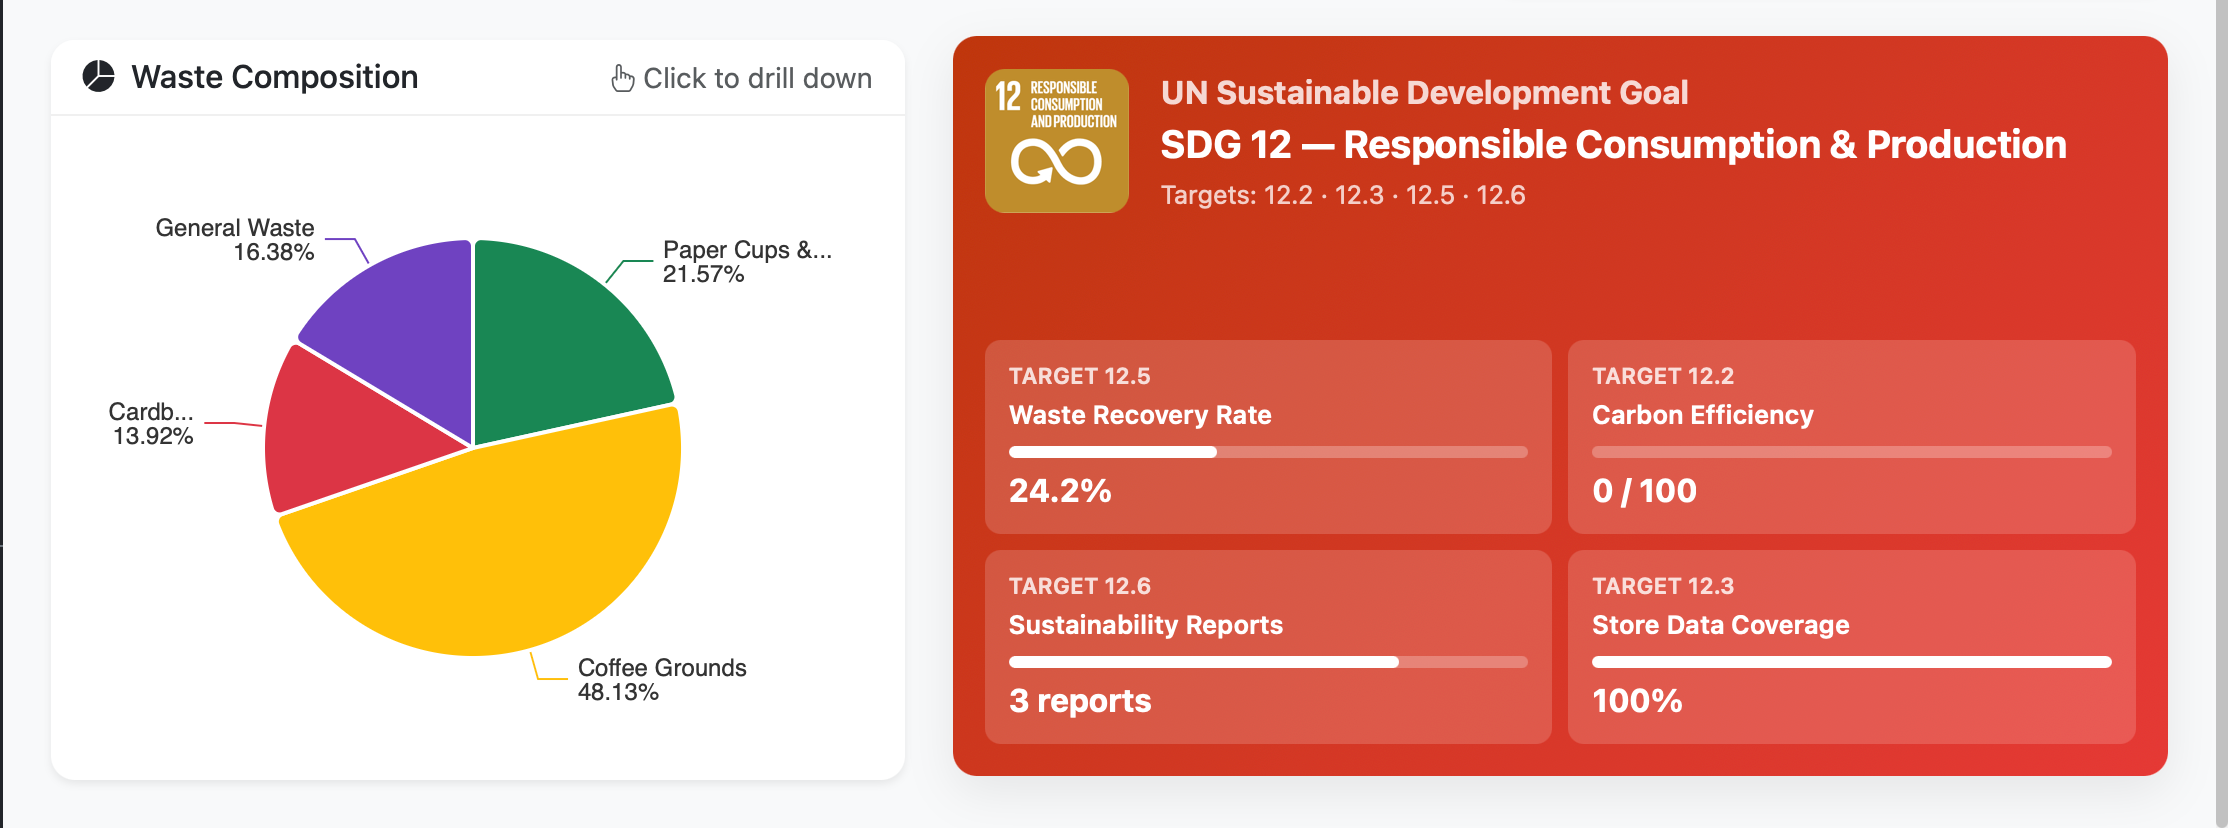
\includegraphics[width=0.50\textwidth]{SDG_panel.png}
  \caption{SDG 12 alignment panel on the dashboard}
  \label{fig:SDG_panel}
\end{figure}

\new{Beyond these shared elements, the dashboard renders an additional role-specific card area below the KPI summary. Store Staff see an \emph{Open Alerts} list scoped to their own store, allowing rapid triage of unread alerts. Region Managers see a \emph{Region Leaderboard} ranking stores within their region by recycling rate and carbon intensity. HQ Managers see a \emph{Risk Watch} card surfacing high-alert stores, carbon-spike stores, and silent (no-data) stores requiring follow-up. Admins additionally see a \emph{System Health} card with active user count, recent audit-log activity, and open alert backlog.}

\begin{figure}[H]
  \centering
  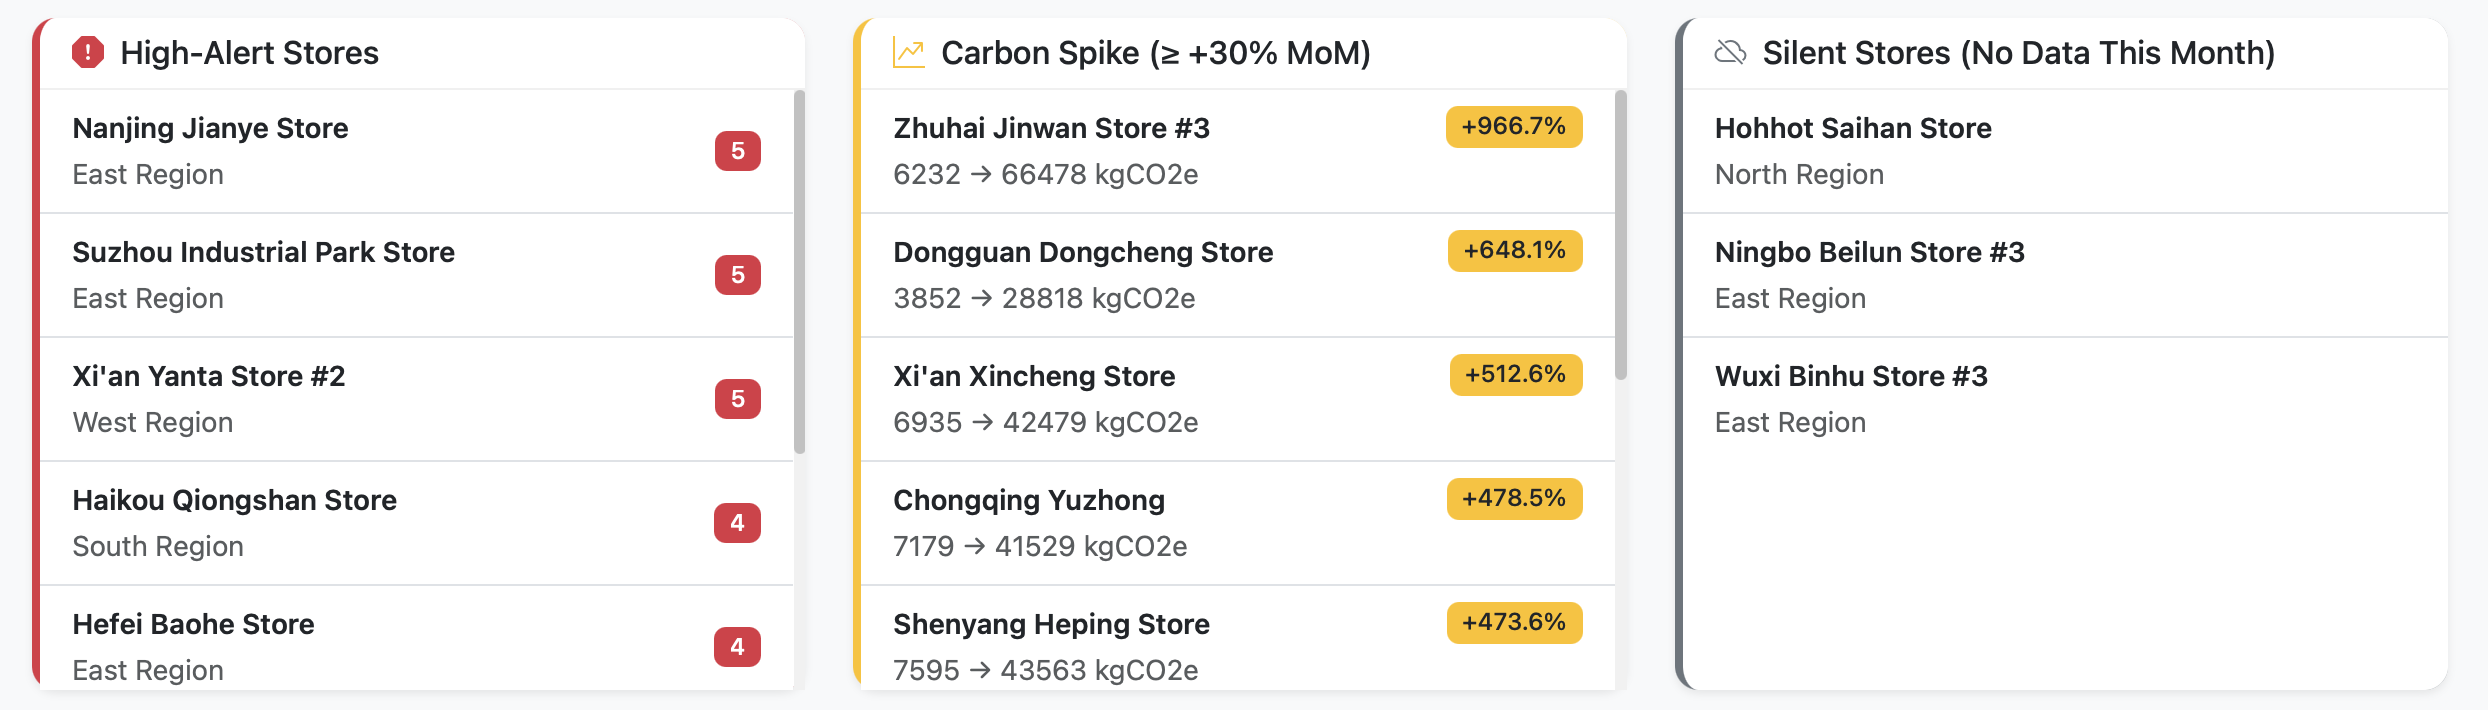
\includegraphics[width=0.92\textwidth]{dashboard_hq_riskwatch.png}\\[0.4em]
  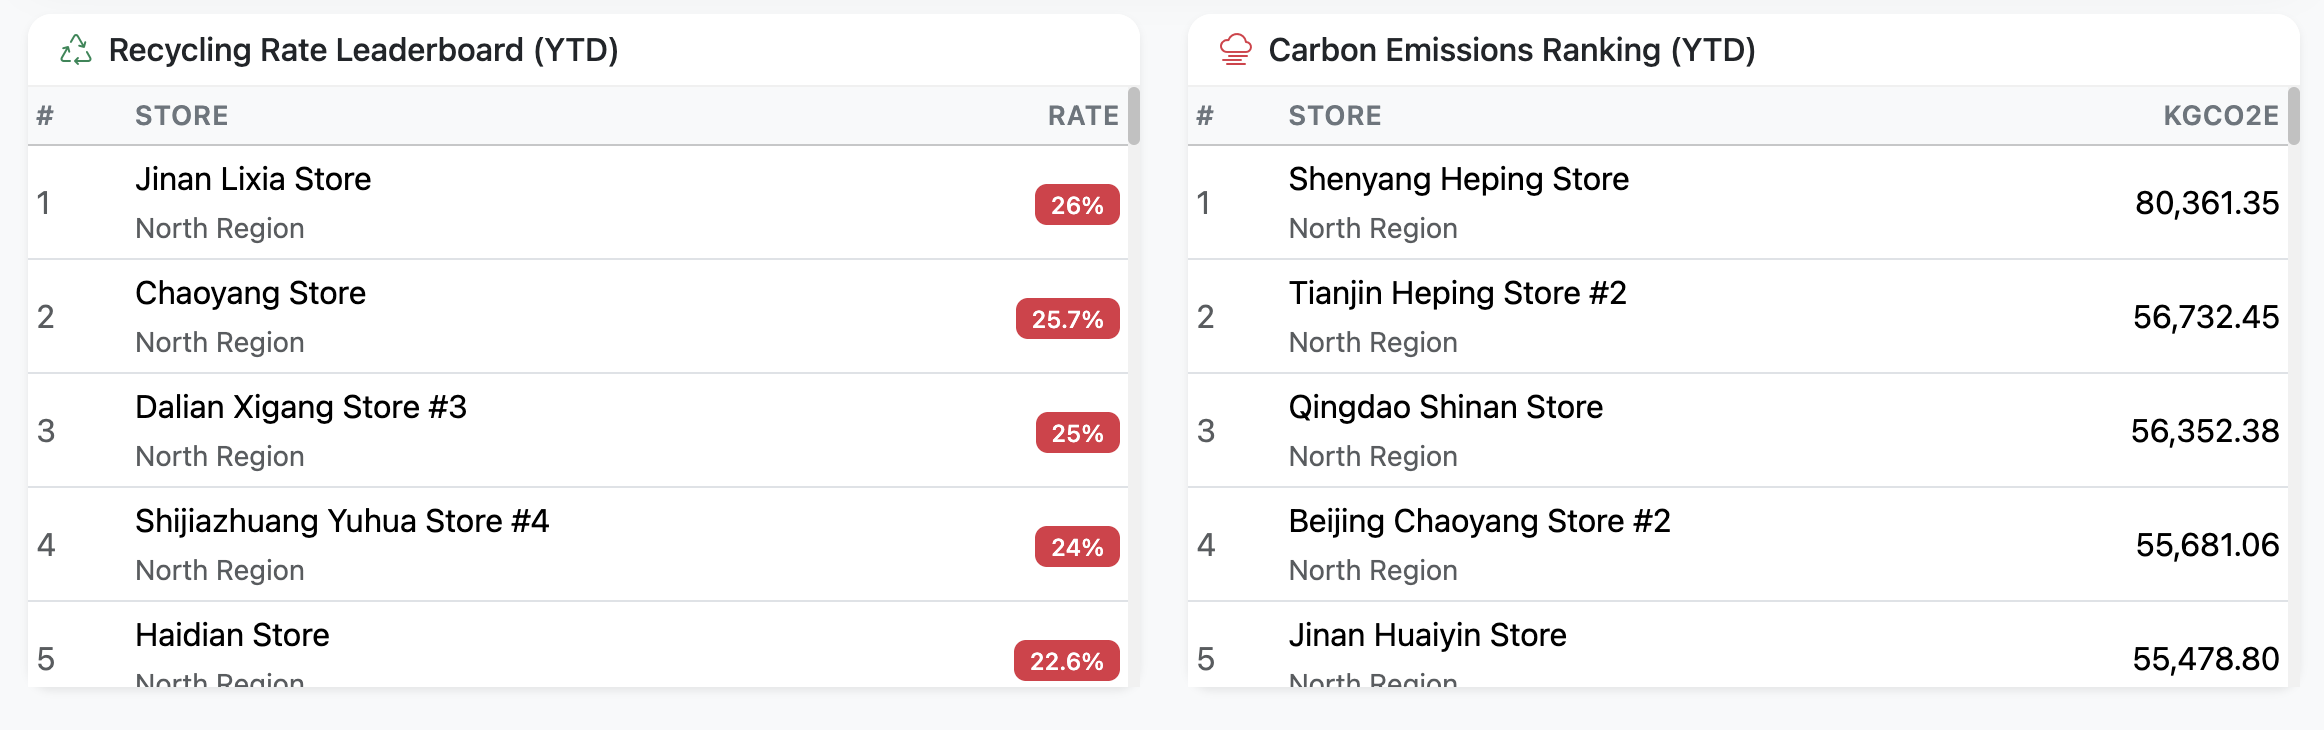
\includegraphics[width=0.92\textwidth]{dashboard_region_leaderboard.png}\\[0.4em]
  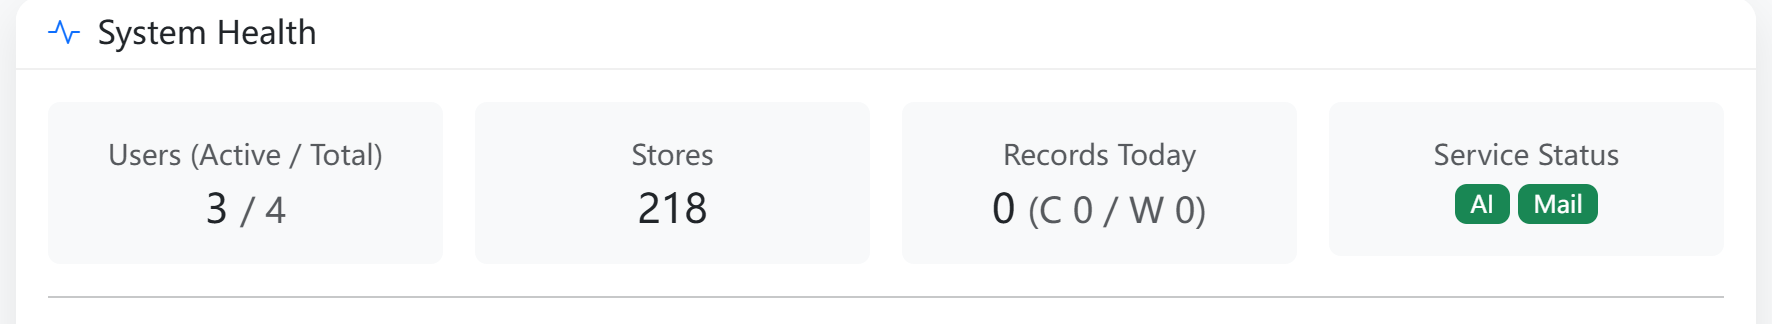
\includegraphics[width=0.92\textwidth]{system_health_card.png}
  \caption{Role-specific dashboard cards. Top: HQ Risk Watch flags high-alert, carbon-spike, and silent stores. Middle: Region Manager Leaderboard ranks stores within the region by recycling rate and YTD carbon emissions. Bottom: Admin System Health card with active-user counts, store count, today's records, and service status. The Store Staff Open Alerts panel is shown in Figure~\ref{fig:staff-view}.}
  \label{fig:role_dashboards}
\end{figure}


\subsection{Carbon Tracking}
The Carbon Tracking page records carbon-related operational activity across the electricity, transport, and fuel categories, with a built-in emission-factor library that auto-computes CO\textsubscript{2}e from the activity value following the factor-based approach of the GHG Protocol~\cite{ghgprotocol} and ISO~14064~\cite{iso14064}. To add an entry, click \emph{Add Record}, fill in the required fields, and submit; the new row appears immediately. \new{The \emph{Scan Bill} button accepts a utility-bill image or PDF and prefills category, activity value, date, and note via OCR}~\cite{tesseract}\new{, with a \emph{Demo Bill} option for testers who do not have a real bill at hand. \emph{Export CSV} downloads the current filtered table, and \emph{Import} accepts CSV or Excel uploads with a downloadable template and per-row error reporting.} Visible data scope follows the user's role, and store staff face tighter edit windows than higher roles. Carbon entries feed downstream dashboards, reports, and compliance scoring.

\begin{figure}[H]
  \centering
  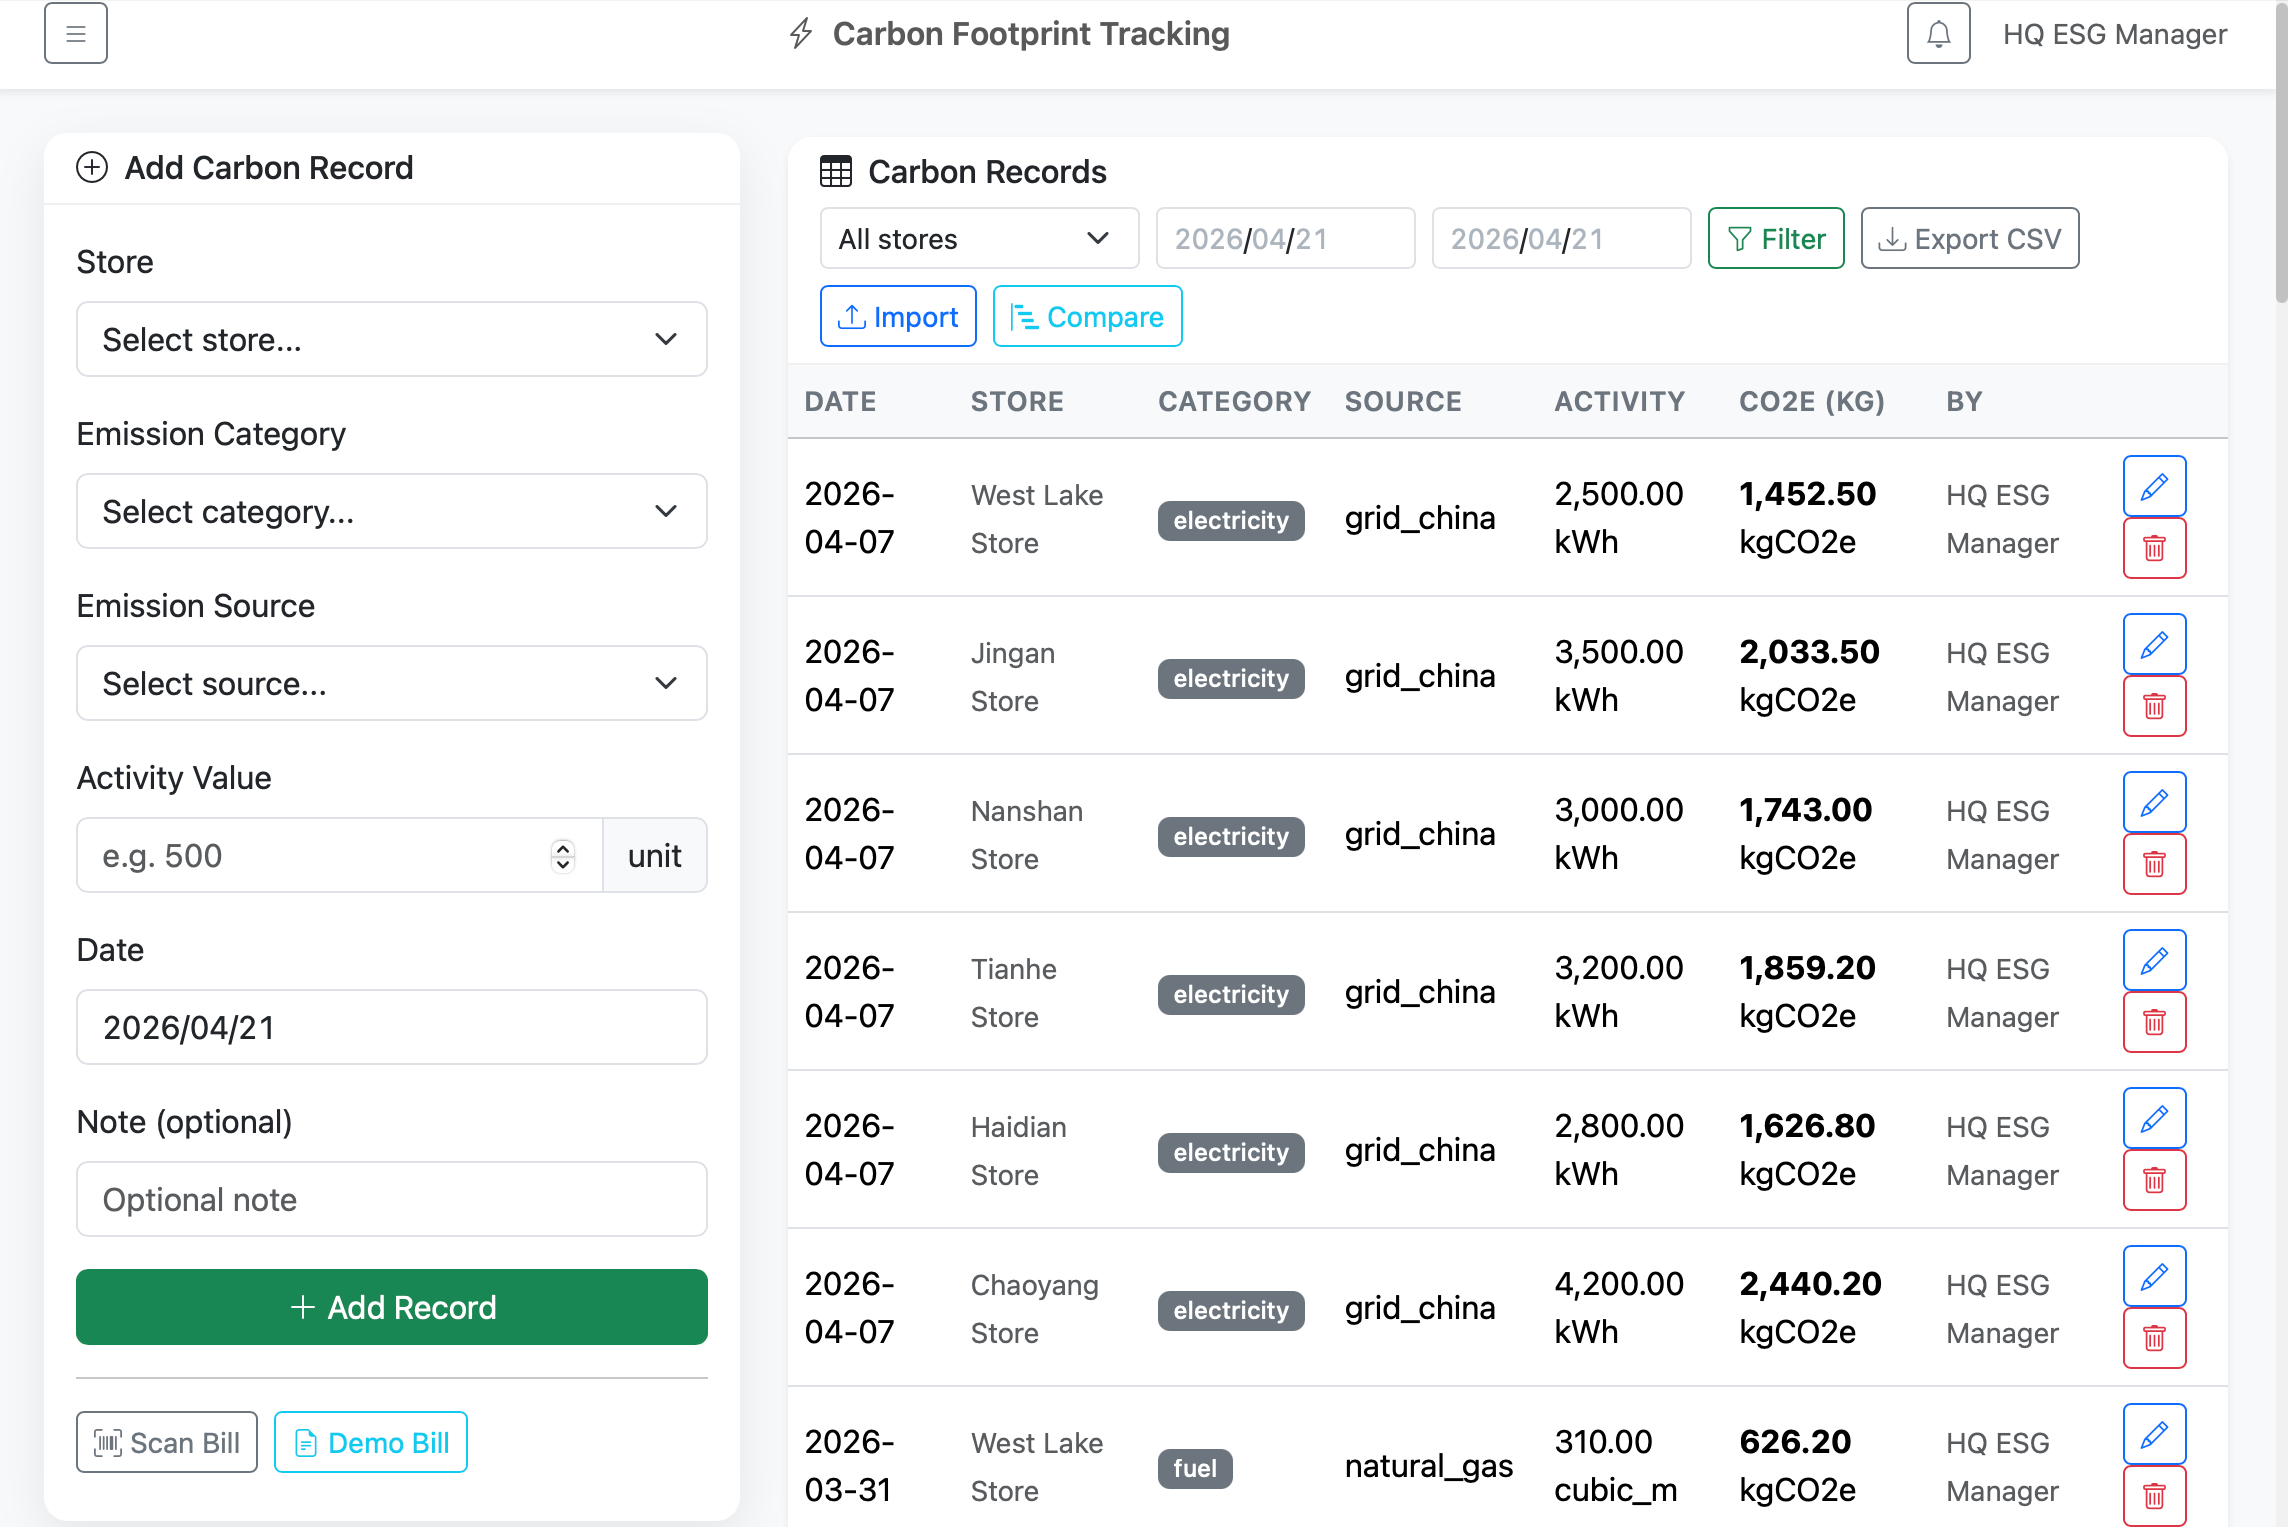
\includegraphics[width=0.60\textwidth]{carbon_tracking.png}
  \caption{Carbon tracking page with the inline entry form and records table}
  \label{fig:carbon}
\end{figure}

\subsection{Waste Management}
The Waste Management page records waste generation and recycling alongside category, source, and disposal information. Supported categories include cup lids, plastic packaging, coffee grounds, food residue, hazardous waste, general waste, cardboard/paper, and e-waste. To log an entry, fill in category, total weight, recycled quantity, source, disposal method, and date, then submit; the system rejects entries where recycled weight exceeds total waste. A \emph{Compare} button opens a month-on-month view that shows this month, last month, and the regional average. \new{Like Carbon Tracking, the page supports CSV/Excel import with template download and per-row validation, plus CSV export of the current filtered view.}

\begin{figure}[H]
  \centering
  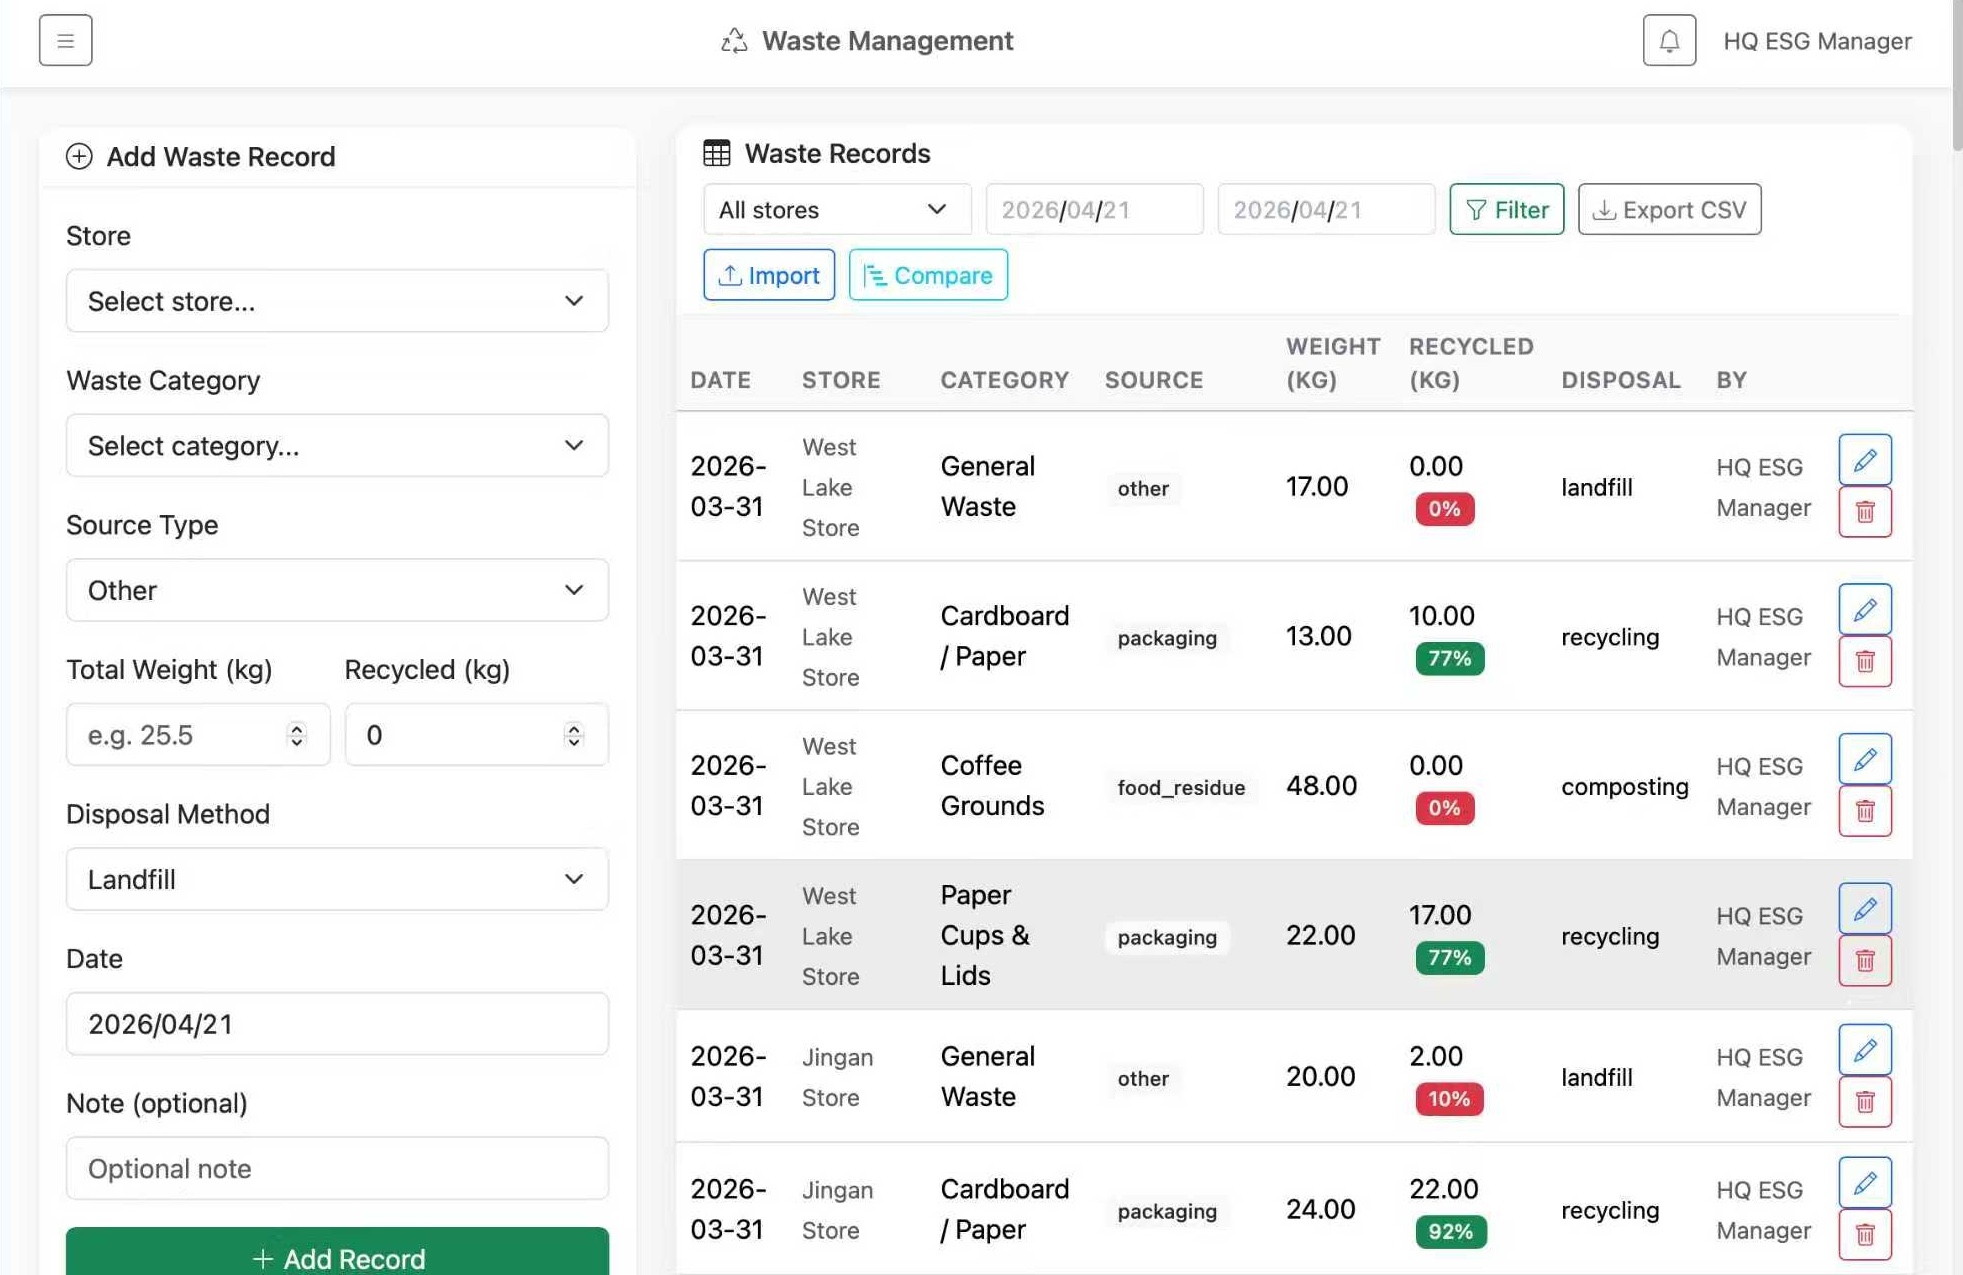
\includegraphics[width=0.60\textwidth]{waste_management.jpg}
  \caption{Waste management page with the inline entry form and records table}
  \label{fig:waste}
\end{figure}

\subsection{Sustainability Reports}
The Reports page generates sustainability reports for a selected time range, in line with standard sustainability reporting practices \cite{gri_standards}. Enter a title, report type, and date range, then click \texttt{Generate Report}. \new{A \emph{Use AI to generate evaluation} switch toggles between an AI-authored ESG analysis powered by the DeepSeek chat-completion API}~\cite{deepseek2024}\new{ and a deterministic rule-based template; the system silently falls back to the template if AI is unavailable and labels the result accordingly.} Generated reports appear in the report list with preview, PDF export, and re-analysis options.

\begin{figure}[H]
  \centering
  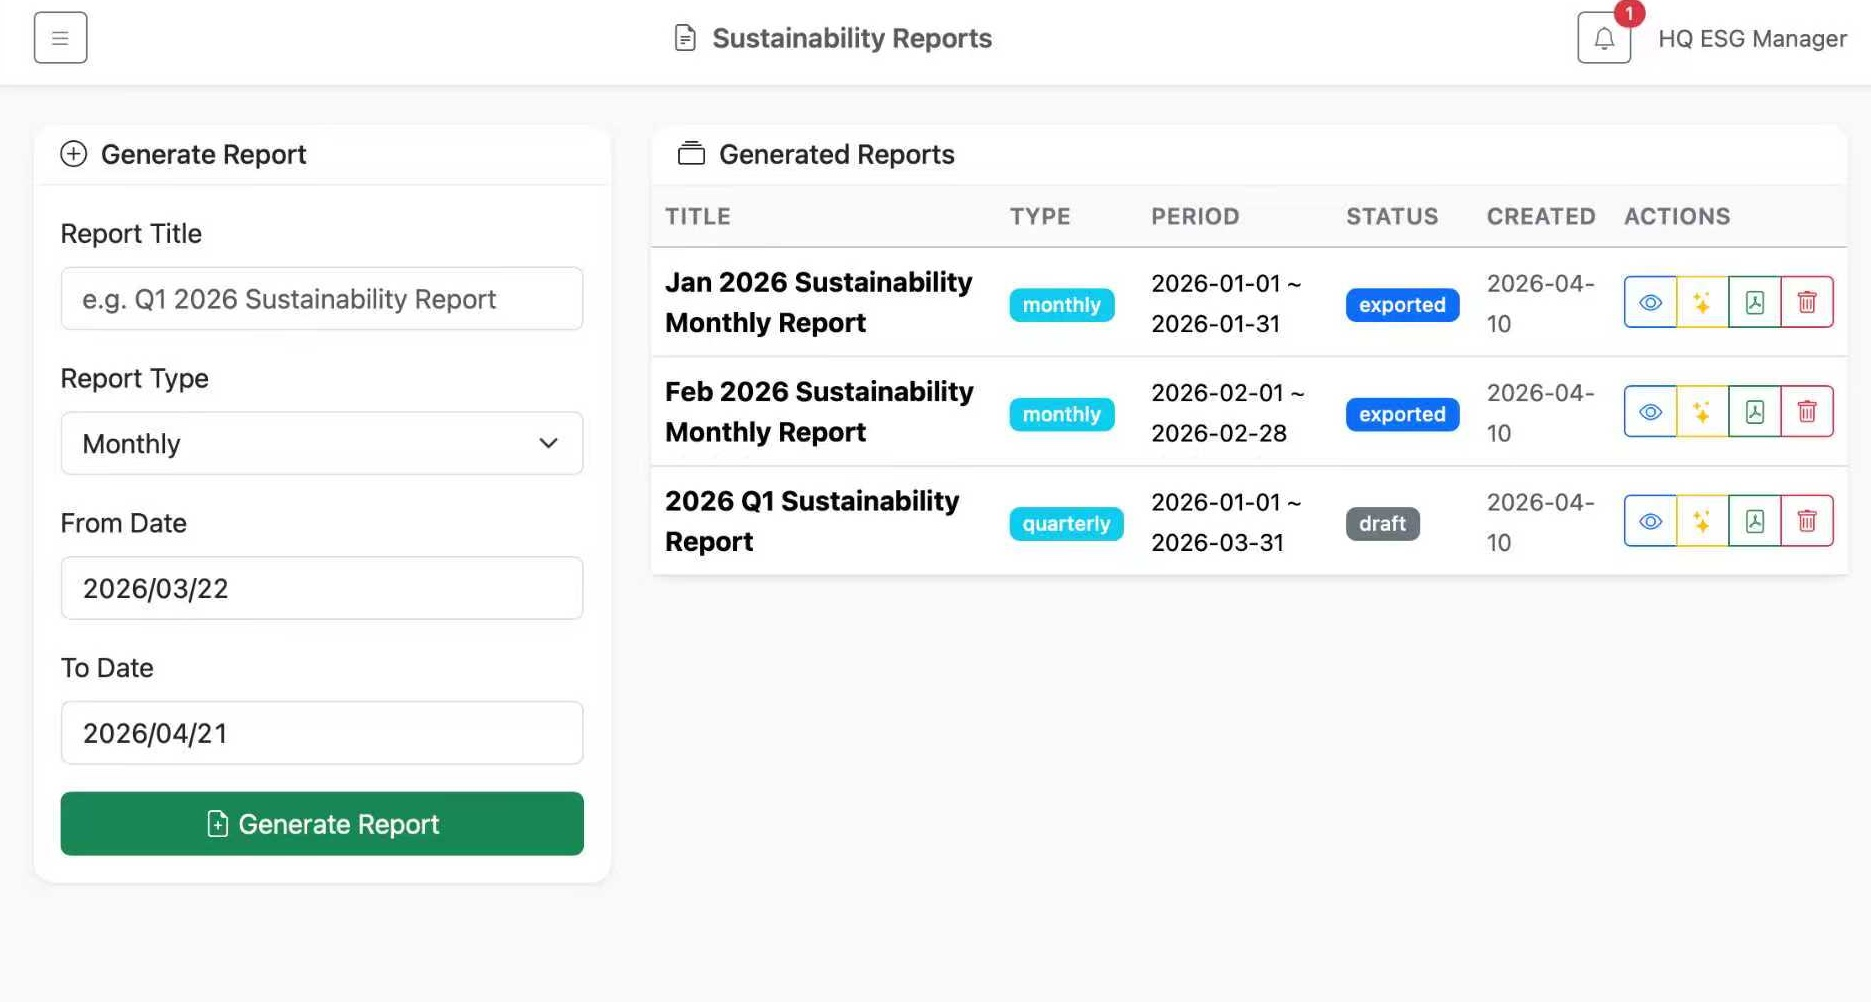
\includegraphics[width=0.65\textwidth]{reports_page.jpg}
  \caption{Sustainability reports page}
  \label{fig:reports_page}
\end{figure}

\subsection{Training Records}
The Training page records staff sustainability training sessions. To log a new session, fill in the course name, type, store, trainee, duration, completion date, score, and status, then submit. Course type and status fields help classify and filter records later. The right panel displays annual summary statistics -- session count, total hours, unique trainees, and average score -- alongside a filterable training-record table.

\begin{figure}[H]
  \centering
  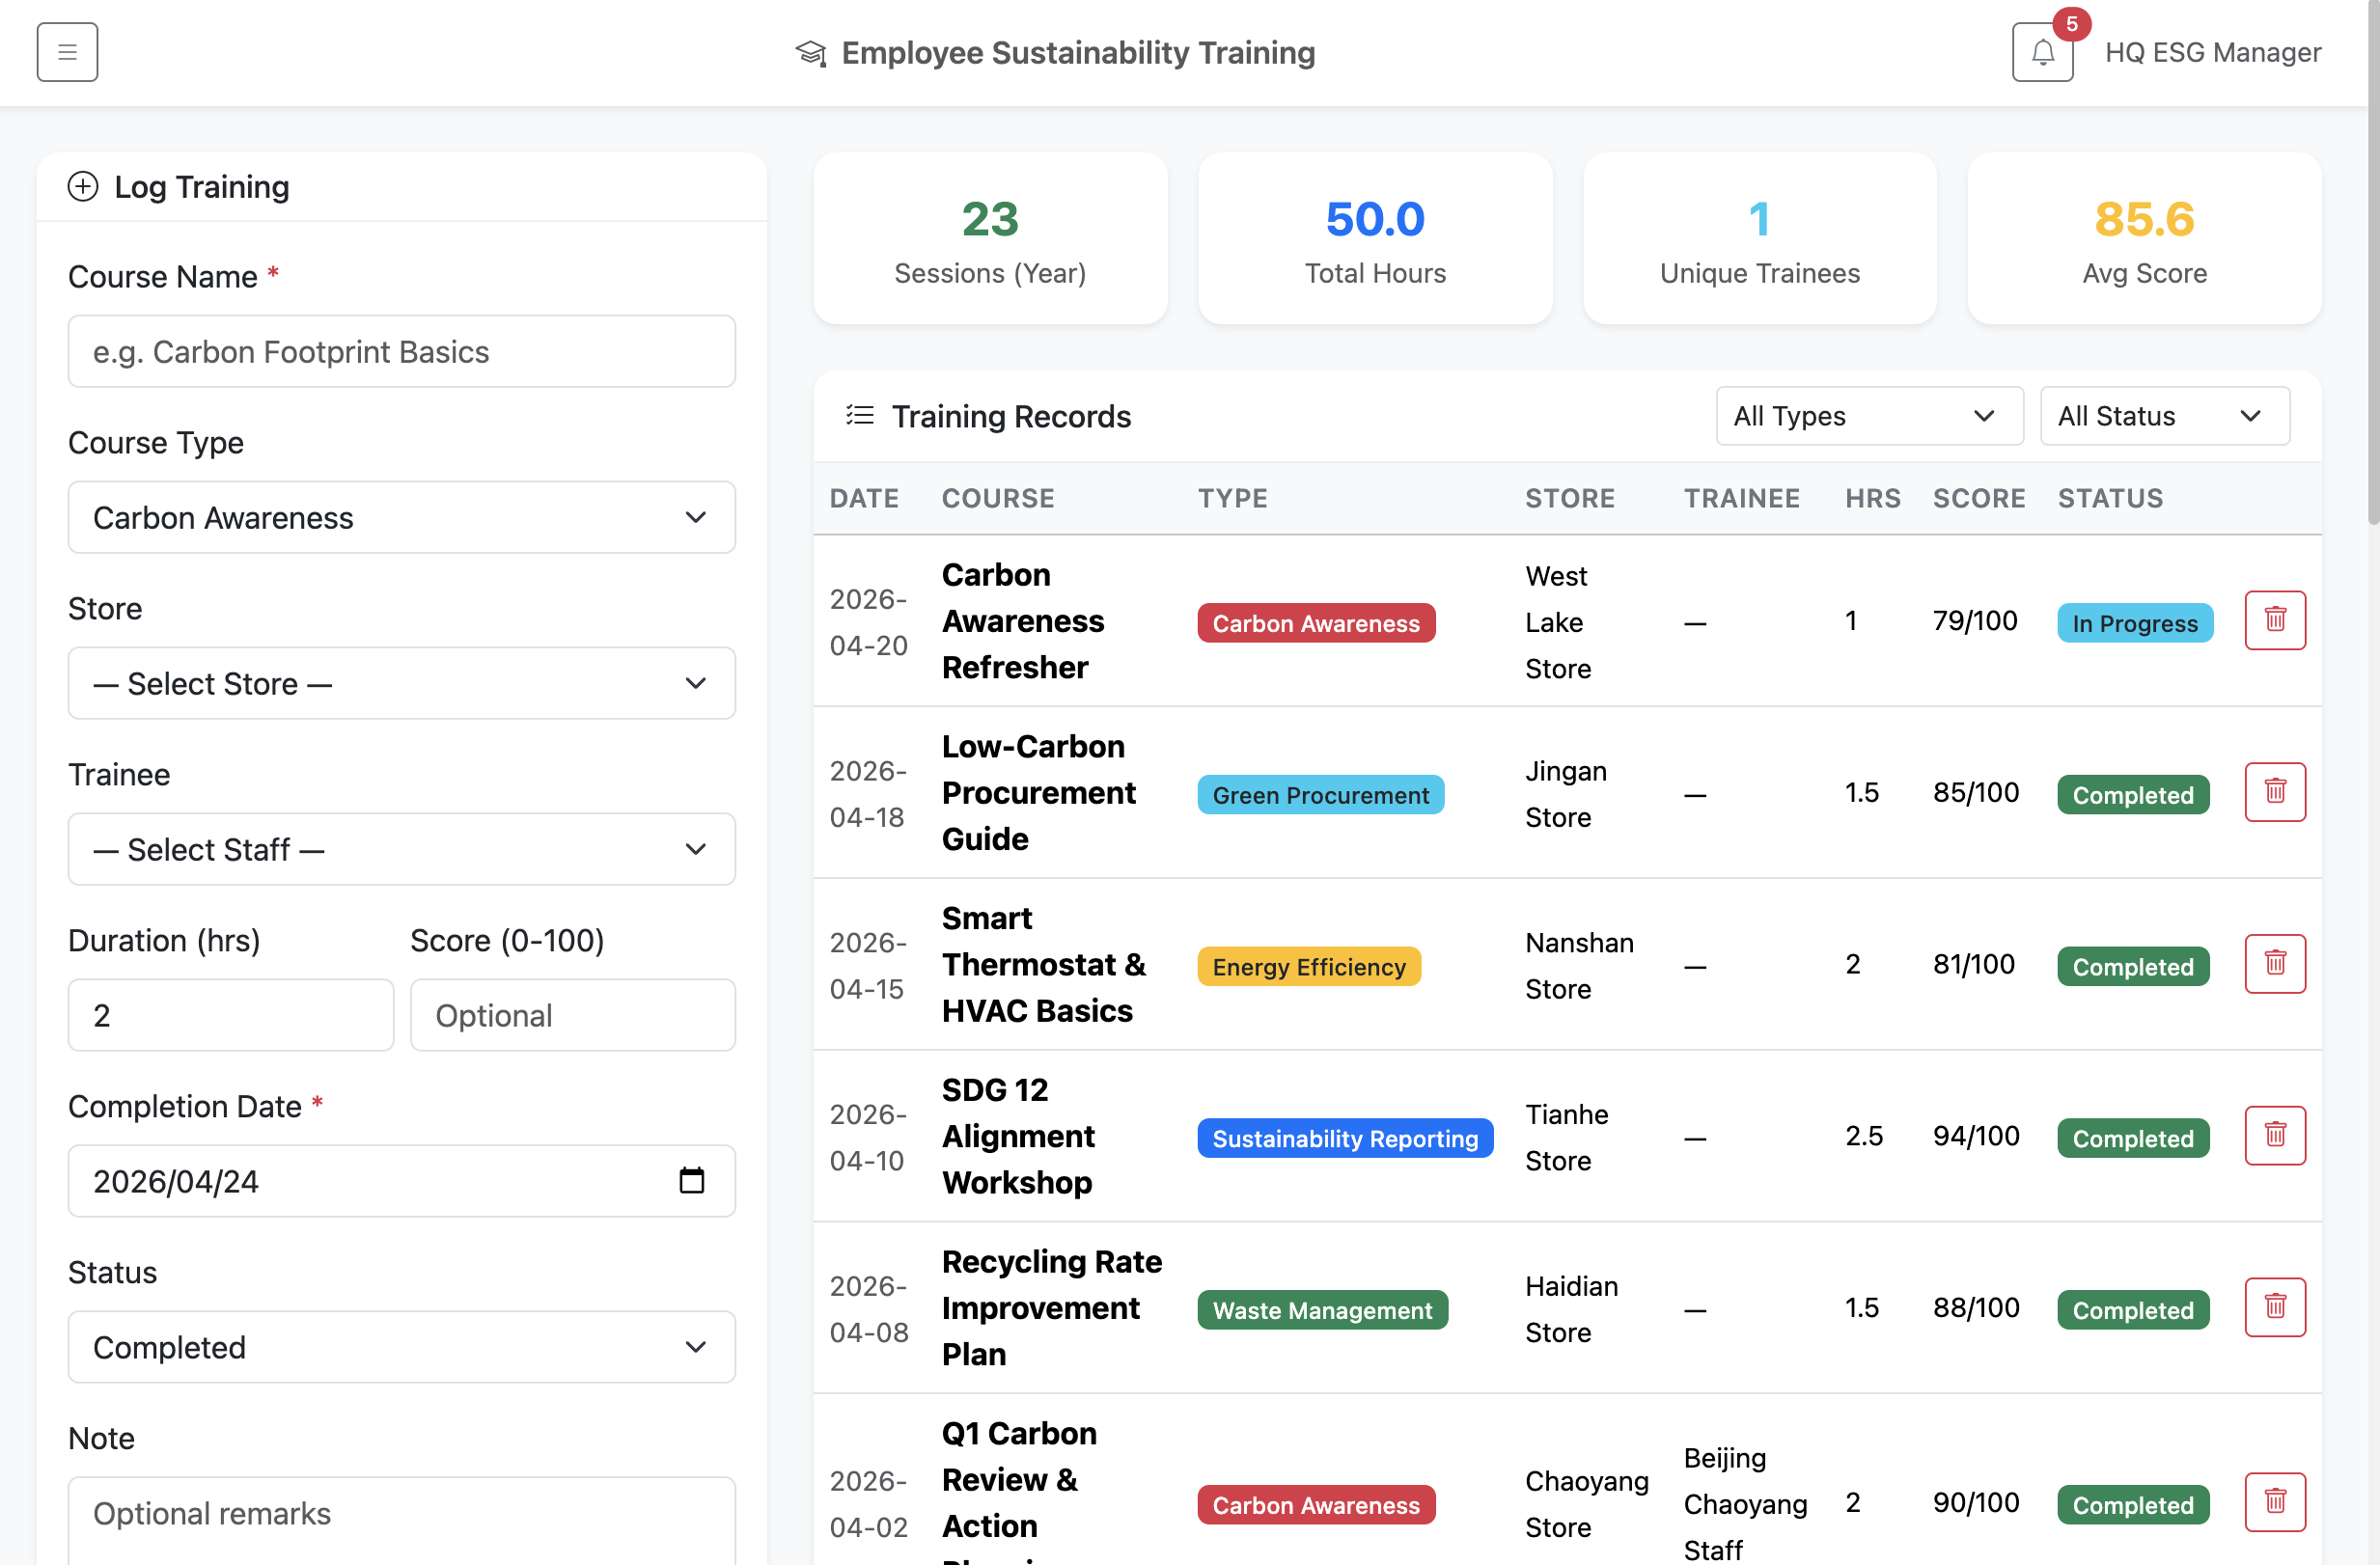
\includegraphics[width=0.85\textwidth]{training_page.png}
  \caption{Training page showing the log form (left), summary statistics, and training records table}
  \label{fig:Training_page}
\end{figure}

\subsection{Store Map}\label{sec:map}
\new{The Store Map page renders accessible stores on an interactive Leaflet}~\cite{leaflet2024}\new{ map and automatically respects the user's data scope -- Store Staff see their own store, Region Managers see their region, and HQ Managers or Admins see the full network. The left-hand sidebar (Figure}~\ref{fig:store-map}\new{) provides a \emph{Map Overview} KPI panel (regions, stores shown, open alerts, total YTD carbon, tree-offset equivalent), a \emph{Quick Search} box, a \emph{View Mode} toggle between individual stores and aggregated regions, a Carbon Heatmap layer, a \emph{Color Markers By} selector (ESG grade, carbon, recovery rate, or open alerts), and Filters covering grade and region. A \emph{Stores Needing Attention} ranking surfaces the worst-performing locations for follow-up, while the map area on the right uses MarkerCluster}~\cite{markercluster}\new{ to group nearby stores at lower zoom levels and reveals individual coloured markers when zoomed in; clicking any marker opens a popup with carbon YTD, recycling rate, and open-alert count.}

\begin{figure}[H]
  \centering
  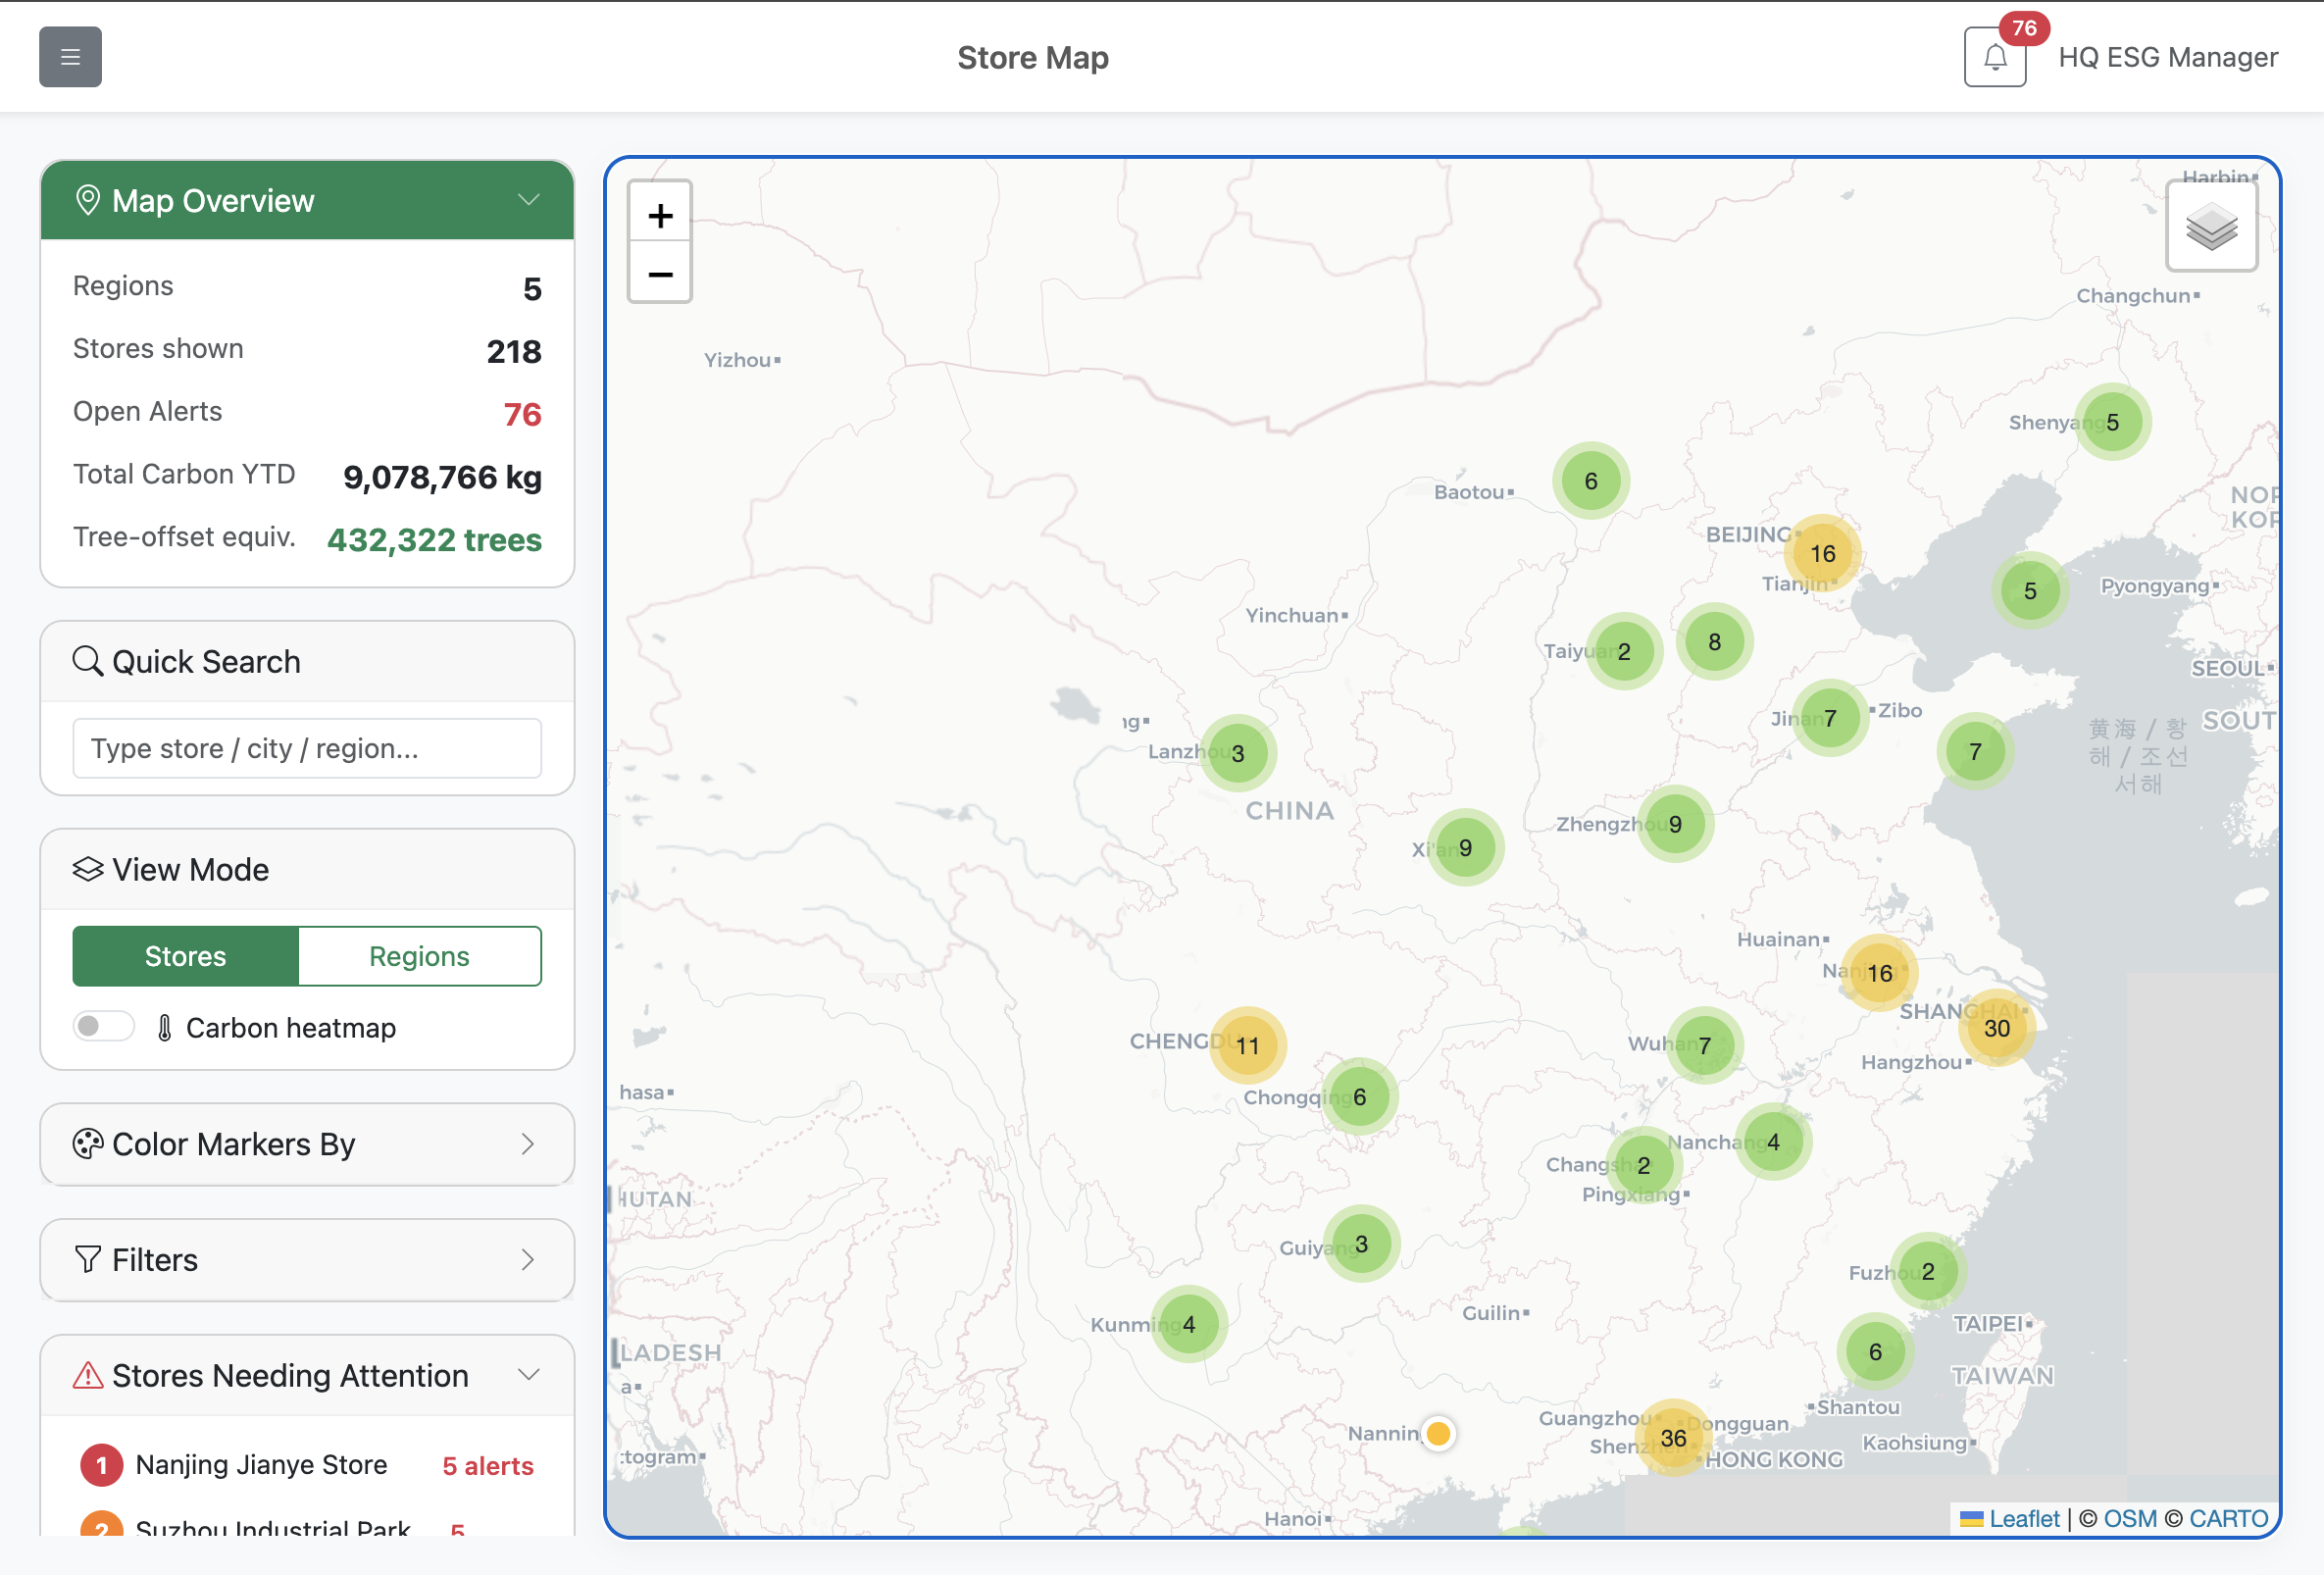
\includegraphics[width=0.92\textwidth]{map_overview.png}
  \caption{Store Map page: KPI summary, Quick Search, View Mode + Carbon heatmap toggle, Color Markers By, Filters, and Stores Needing Attention panel on the left, with clustered store markers rendered over the regional map on the right.}
  \label{fig:store-map}
\end{figure}


\section{Store Staff Guide}

Store staff are the most operationally focused users on the platform. Their primary responsibility is to record day-to-day sustainability data for their own store, contributing to consistent data collection across the organisation. The main pages used by store staff are Dashboard, Carbon Tracking, Waste Management, Reports, and Training.

A typical store staff workflow begins by reviewing the dashboard after login, then entering new carbon records for ongoing store operations, followed by waste records with accurate recycling values. Reports can be generated or reviewed as needed for the current period, and training activities can be logged or checked at any time.

Store staff do not have access to threshold configuration, compliance scoring, anomaly detection, user management, or audit logs. Their visible data is restricted to their own store, and edit or delete operations on submitted records may be subject to stricter time limits than higher-level roles.

\begin{figure}[H]
  \centering
  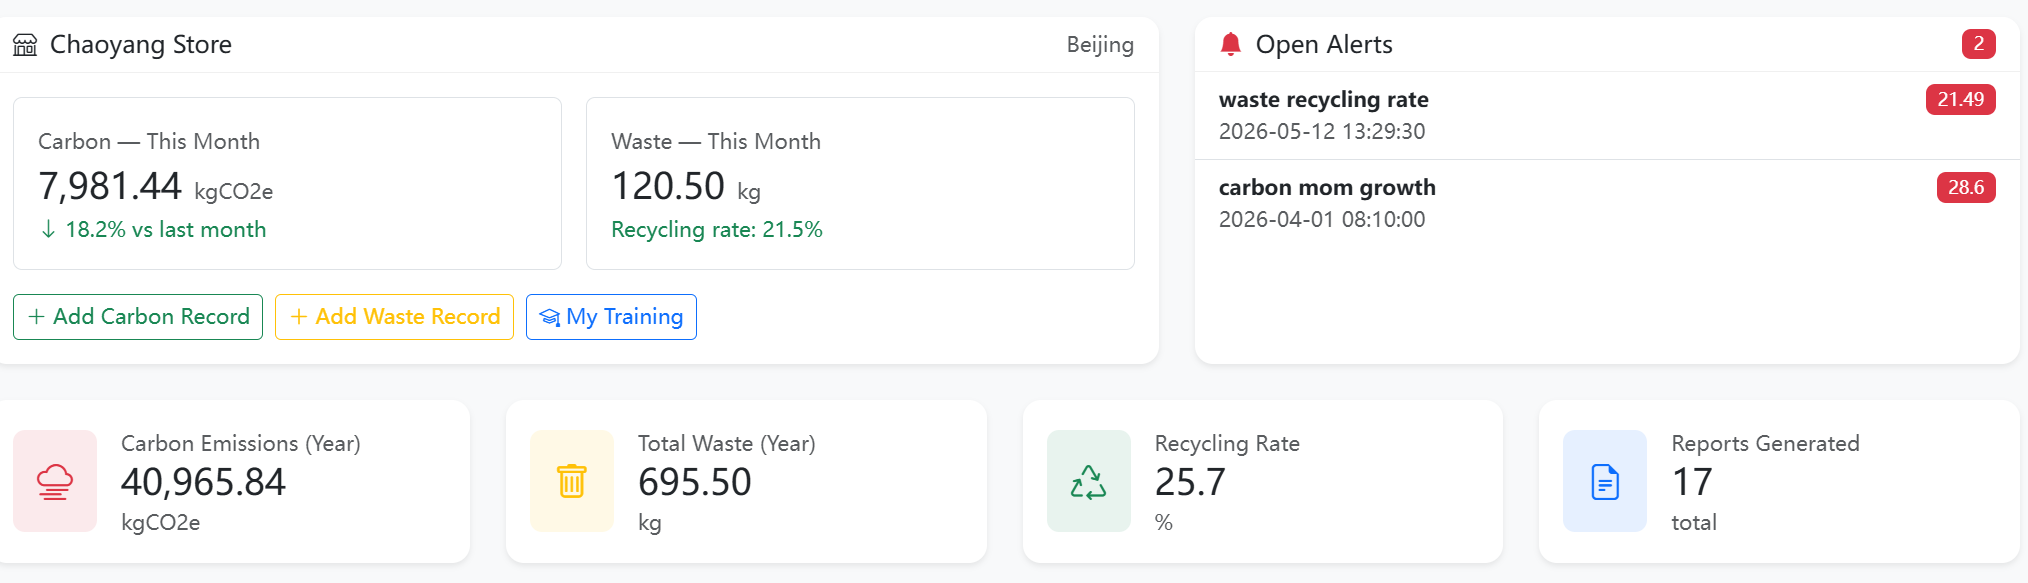
\includegraphics[width=0.62\textwidth]{dashboard_staff_v2.jpg}\\[0.4em]
  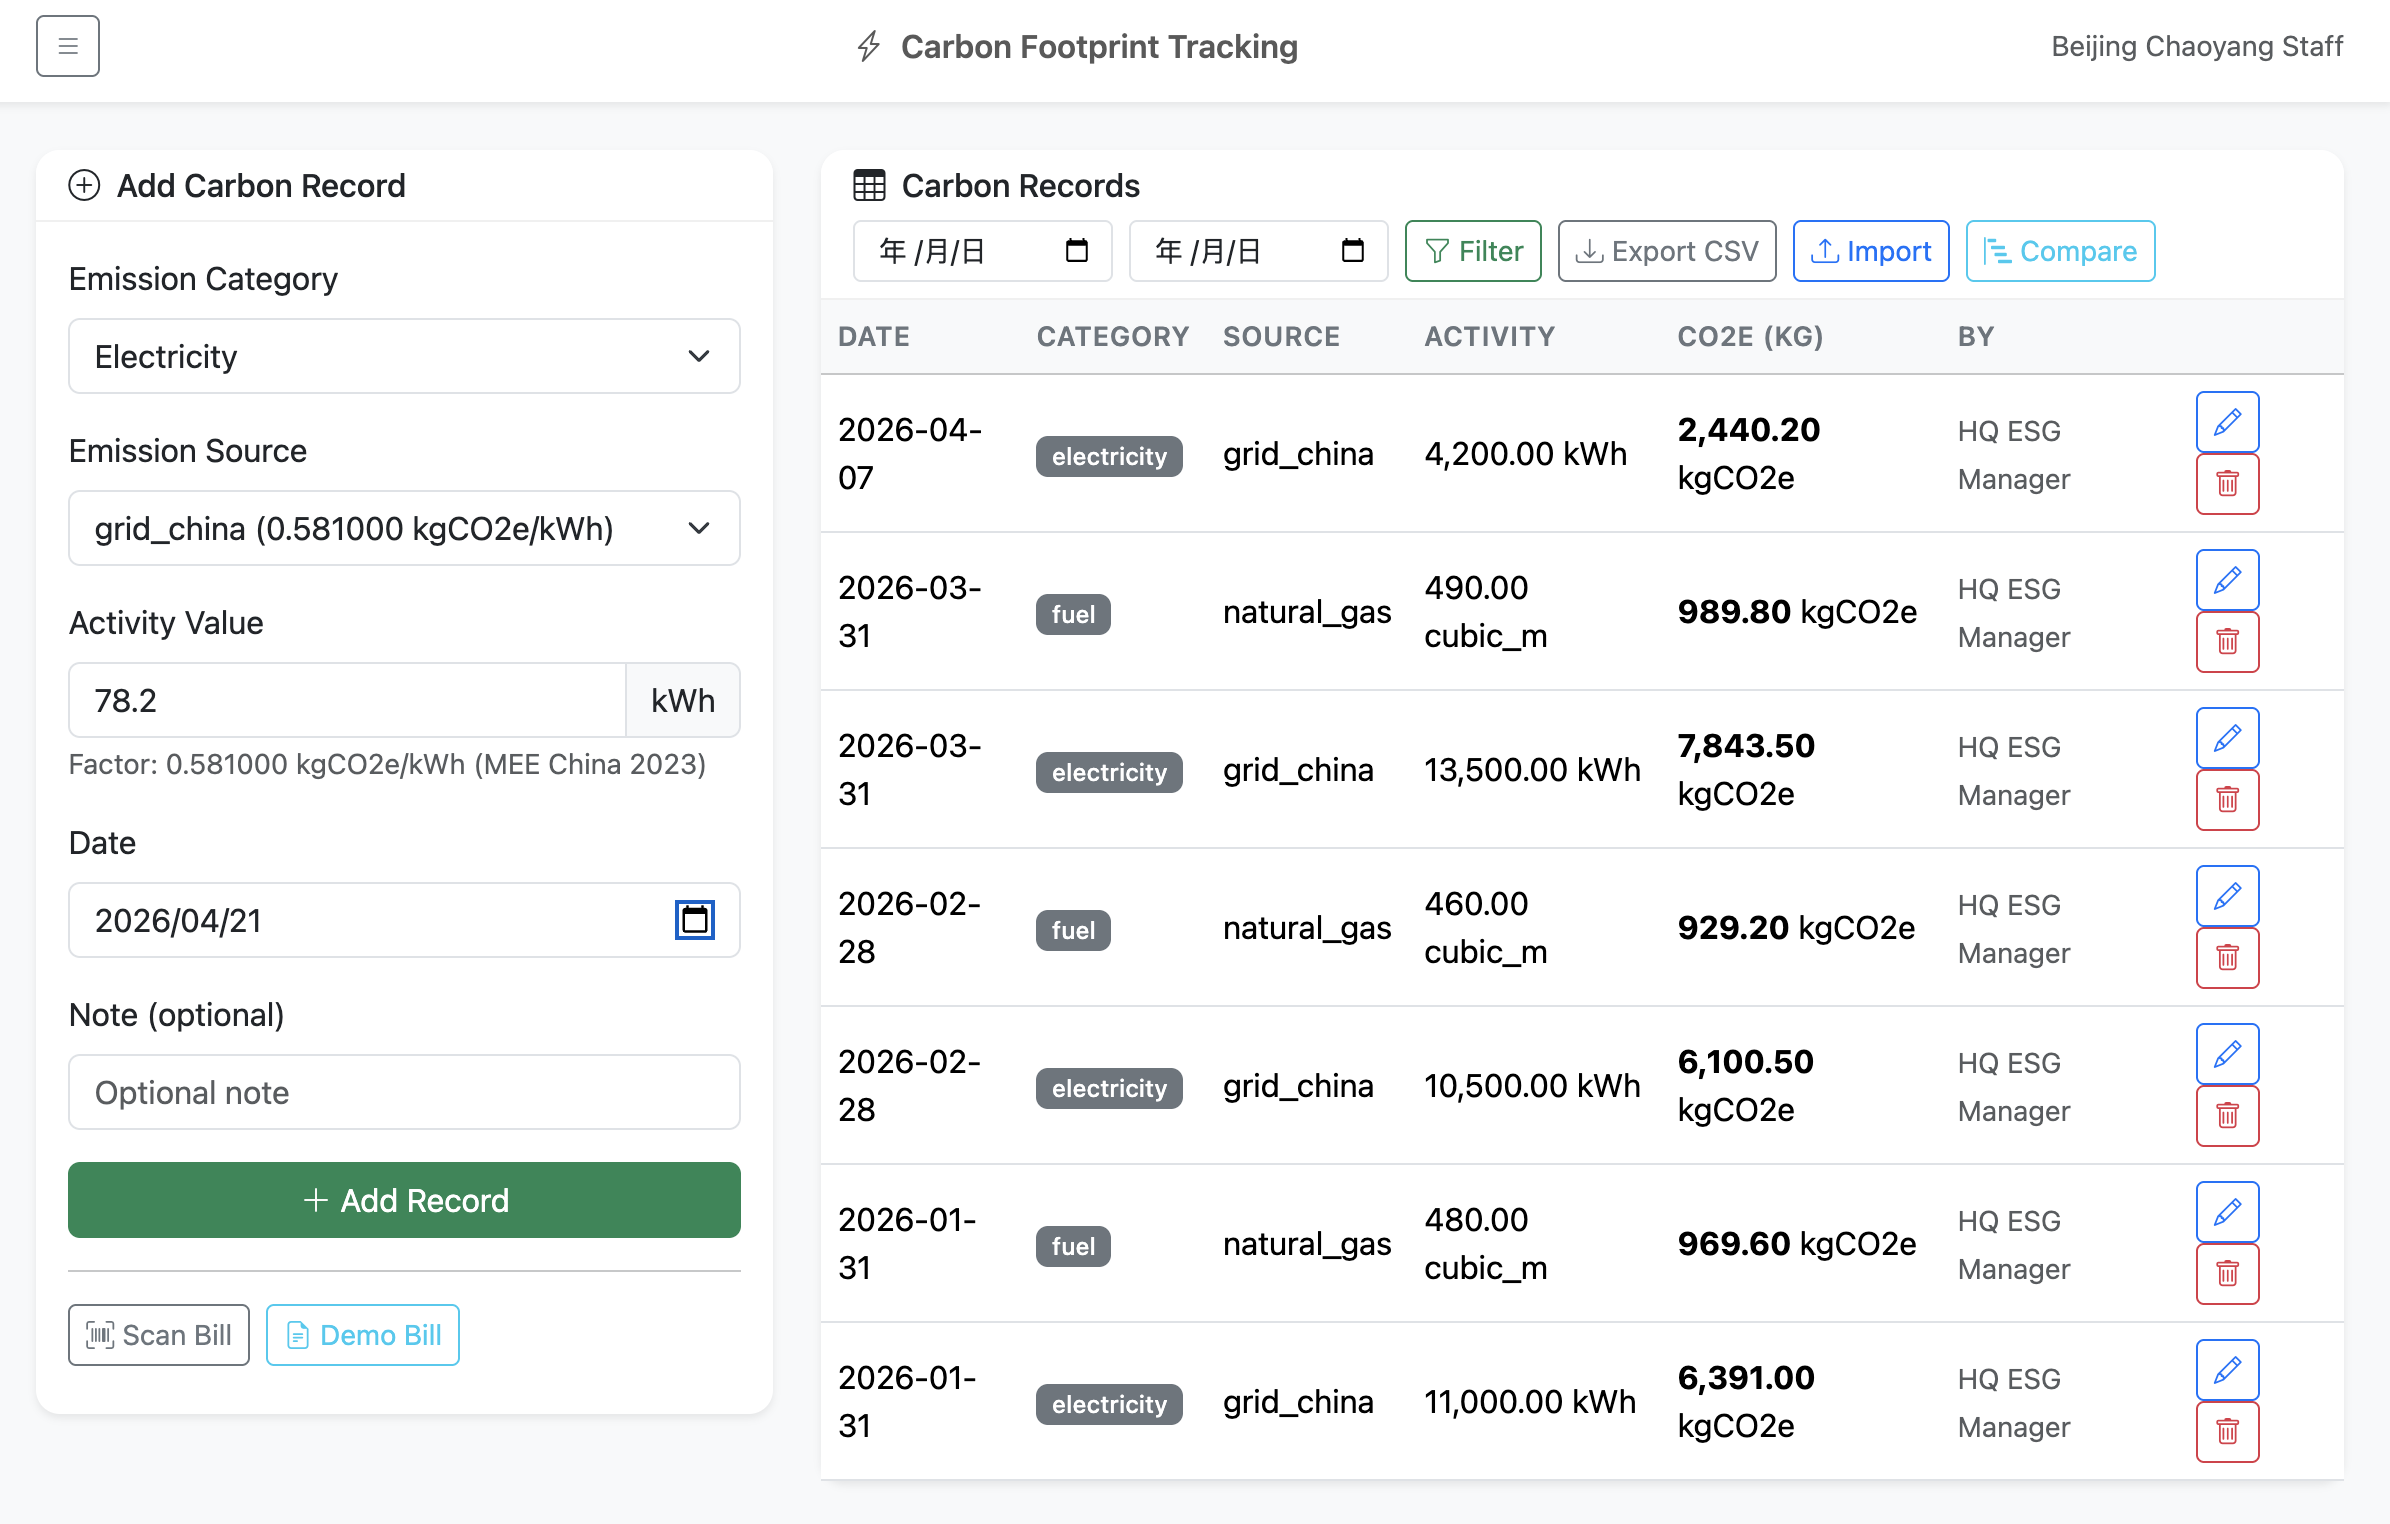
\includegraphics[width=0.85\textwidth]{carbon_add_form.png}
  \caption{Store staff dashboard with KPI cards and the Open Alerts panel (top), and the carbon record entry form (bottom)}
  \label{fig:staff-view}
\end{figure}


\section{Region Manager Guide}
\label{sec:region}

Region managers supervise sustainability performance across multiple stores within their assigned region. Compared with store staff, they focus less on raw data entry and more on monitoring, comparison, and issue identification. In addition to the common pages, region managers can access the Alerts page (described in Section~\ref{sec:alerts-config}) for log review, the Compliance Score page, and Anomaly Detection -- together helping them identify unusual values, assess ESG readiness, and monitor whether stores are meeting sustainability expectations.

\subsection{Compliance Score Page}
The Compliance Score page allows management users to calculate and review an ESG scorecard for a selected year. It includes an overall score gauge, a grade label, dimension breakdowns, and detailed metric rows. This page helps managers translate many separate sustainability activities into one structured review surface.

\begin{figure}[H]
  \centering
  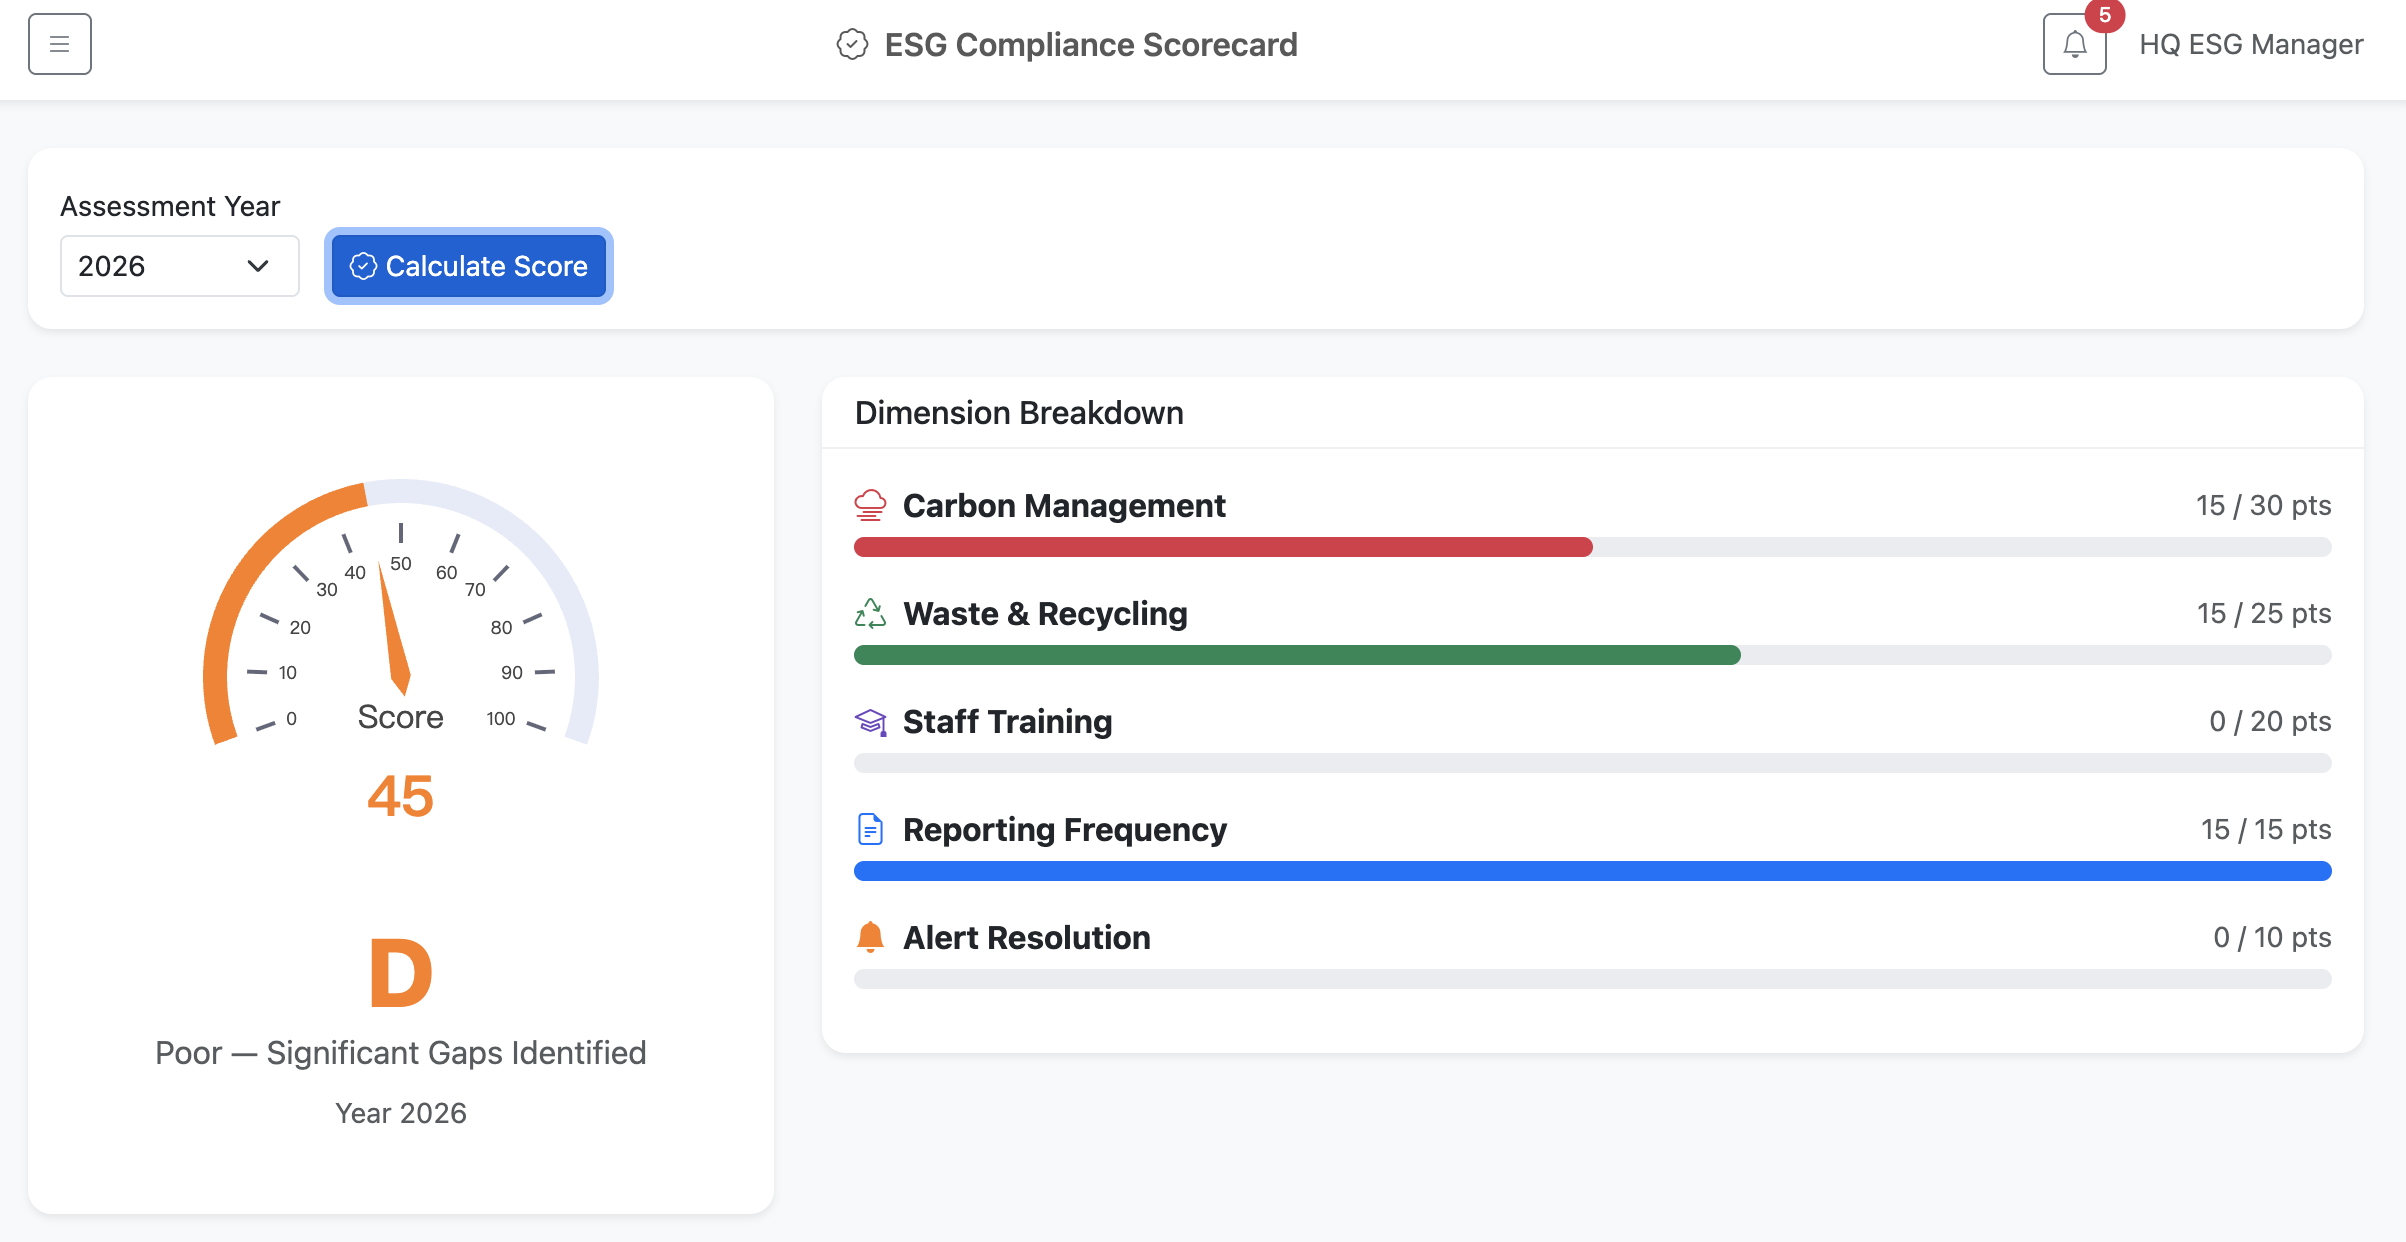
\includegraphics[width=0.65\textwidth]{compliance_score.png}
  \caption{Compliance Score page showing ESG scorecard and dimension breakdown}
  \label{fig:compliance_score}
\end{figure}

\subsection{Anomaly Detection}
The Anomaly Detection page flags suspicious carbon and waste values using Z-score deviation~\cite{chandola2009} (with a user-adjustable threshold from 1.5\,$\sigma$ to 3.0\,$\sigma$) combined with hard rules such as non-positive emissions or recycled weight exceeding total weight. \new{For each category, the top three anomalies receive an AI-authored analysis covering likely cause, risk category, and recommended actions, produced via the DeepSeek chat-completion API}~\cite{deepseek2024}\new{ with a deterministic template fallback when AI is unavailable.} Region managers verify a flagged record by cross-referencing the original entry in Carbon Tracking or Waste Management; \new{each anomaly can then be marked as Reviewed, False Positive, or Resolved, and the review state persists across subsequent detection runs to avoid re-investigating already-resolved cases.} Genuine data errors should be corrected by the relevant store staff, while repeated anomalies for a single store warrant escalation to an HQ manager.

\begin{figure}[H]
  \centering
  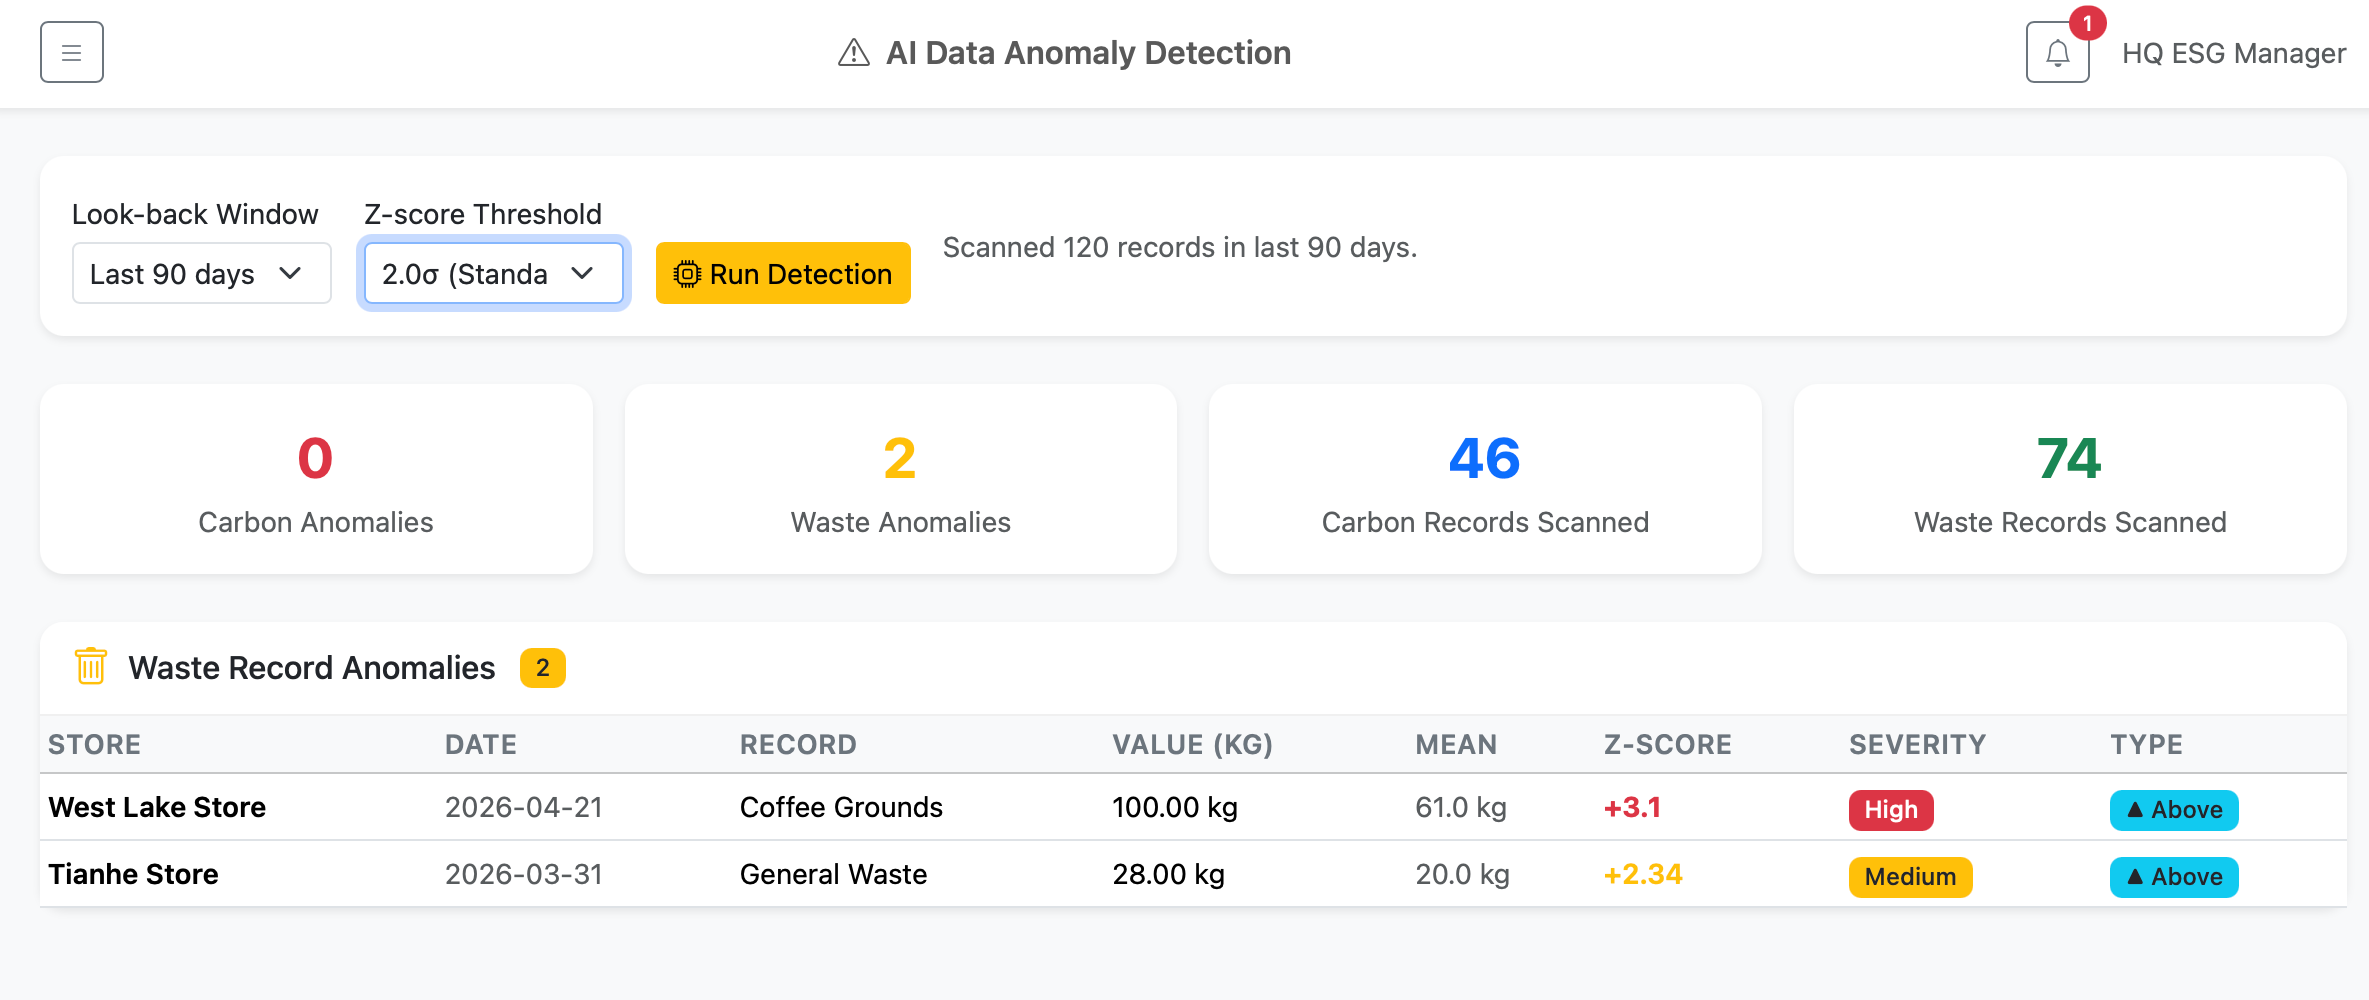
\includegraphics[width=0.80\textwidth]{anomaly_detection.png}
  \caption{Anomaly Detection page with flagged records}
  \label{fig:anomaly_detection}
\end{figure}

\section{HQ Manager Guide}\label{sec:hq}

HQ managers operate at the company level and are responsible for governance-oriented and configuration tasks. Their work supports the broader idea that organisational sustainability performance depends on consistent measurement, monitoring, and accountability~\cite{eccles2014}. After login, an HQ manager typically begins by reviewing the dashboard, then checks the Alerts page for any threshold breaches, reviews the Compliance Score page, and follows up with supplier ESG scores and internal policy status.

\subsection{Alert Threshold Configuration}\label{sec:alerts-config}
The Alerts page serves both region managers and HQ managers. Region managers review alert logs, inspect metric values, and mark items as read. HQ managers additionally define threshold rules through a form covering metric type, condition, threshold value, scope, and an optional notification email. \new{Each new carbon or waste record is checked against the active rules: breaches are written to the alert log, surface as an unread-count badge on the Alerts navigation item (auto-refreshed every 60 seconds), and trigger an email to the configured address -- with a server-log fallback when SMTP is not configured, so demo environments still produce a visible audit trail.}
\begin{figure}[H]
  \centering
  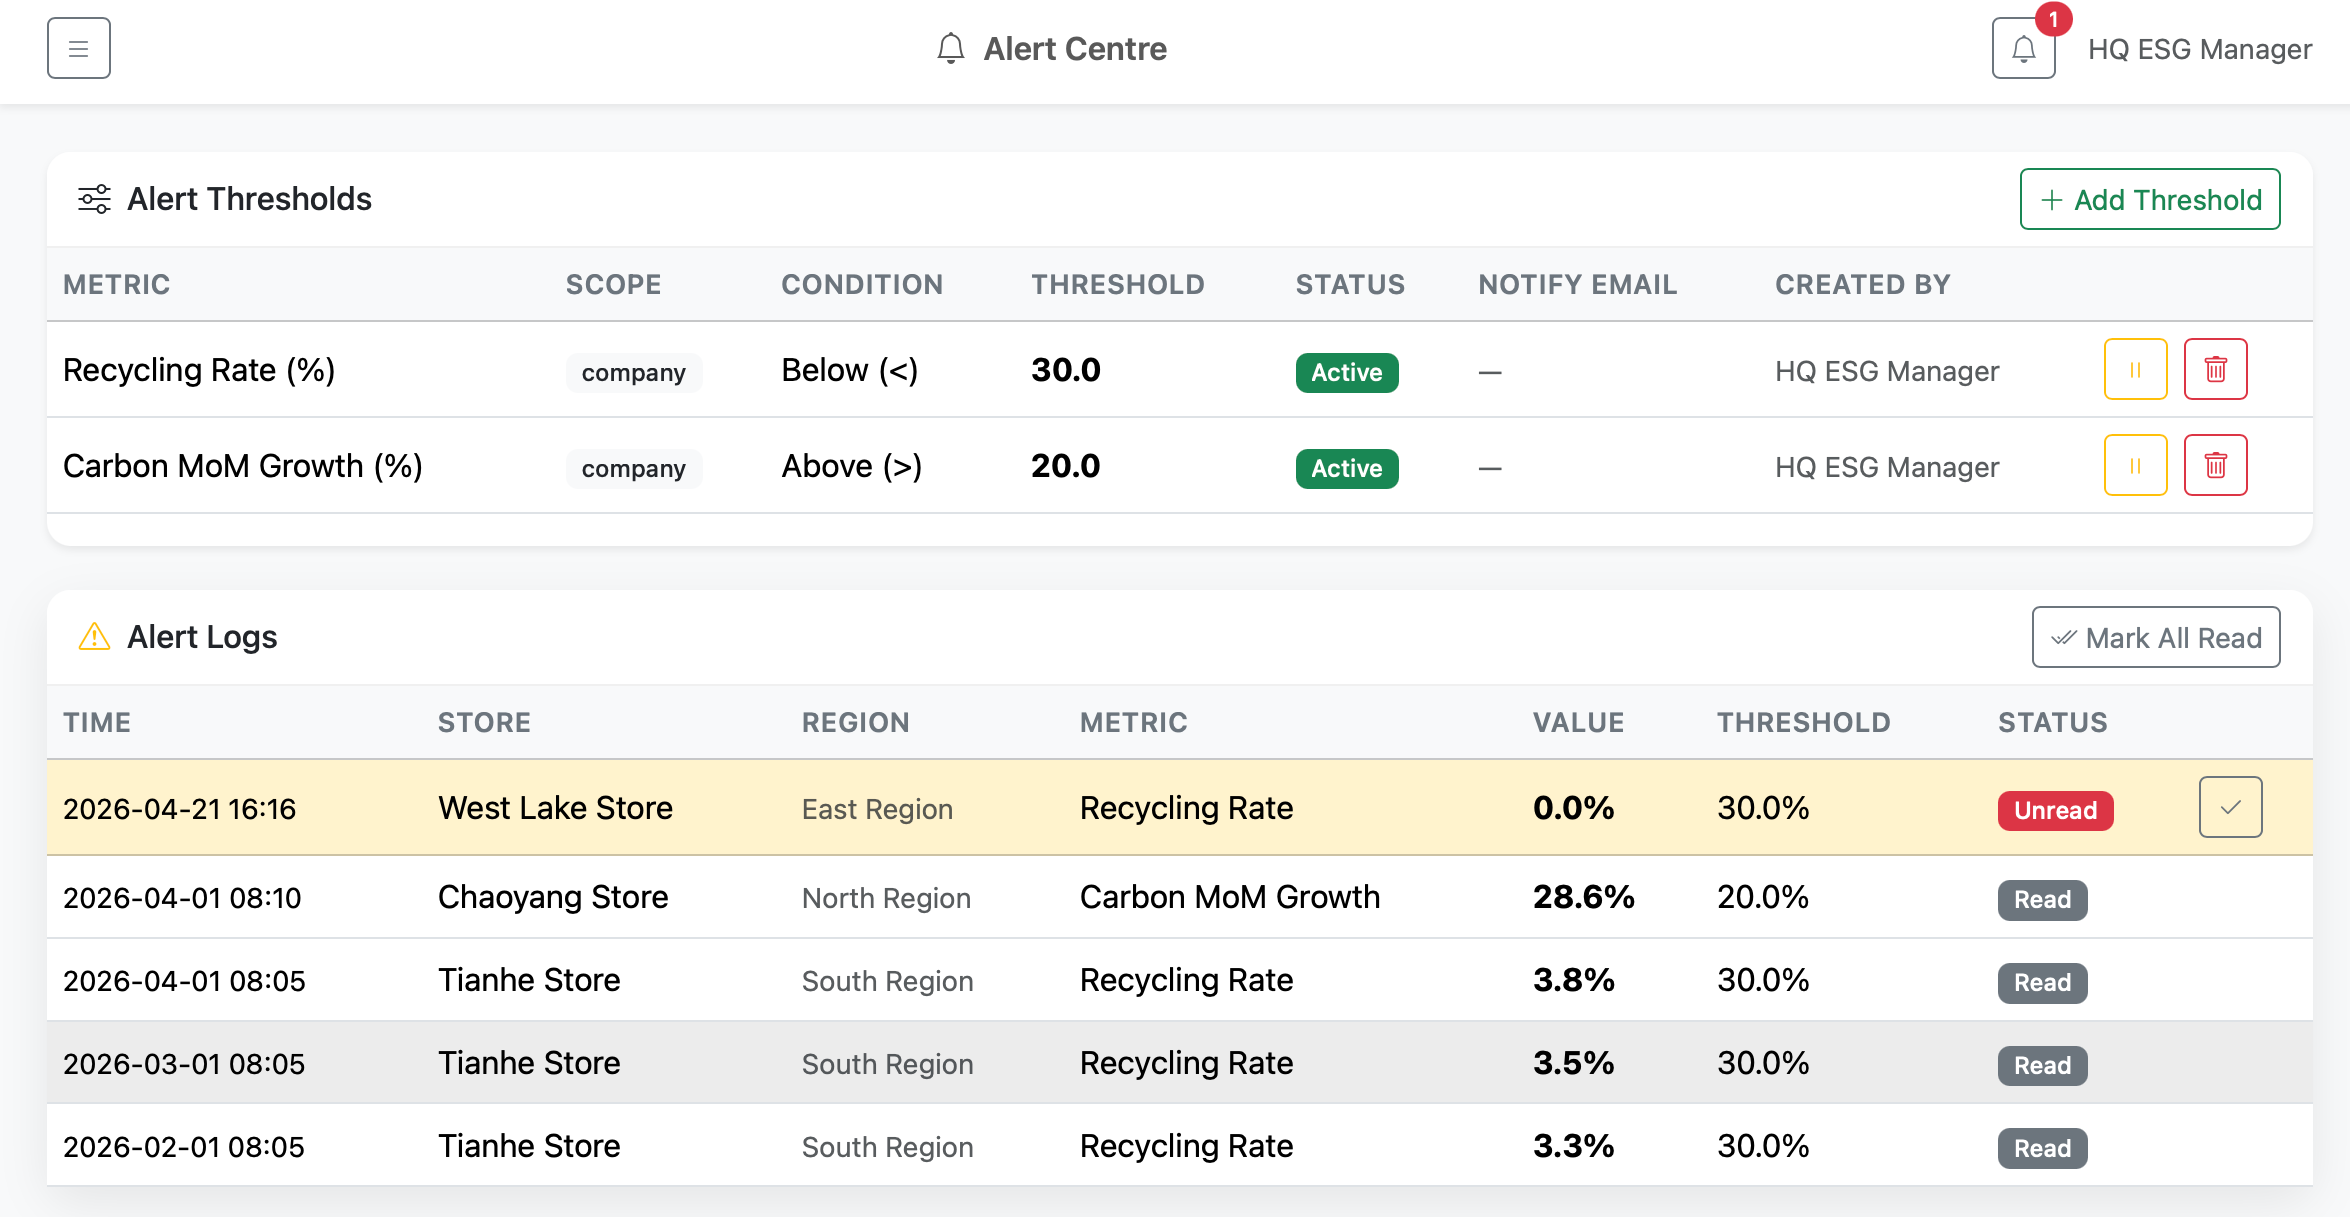
\includegraphics[height=5.5cm]{alert_page.png}
  \hfill
  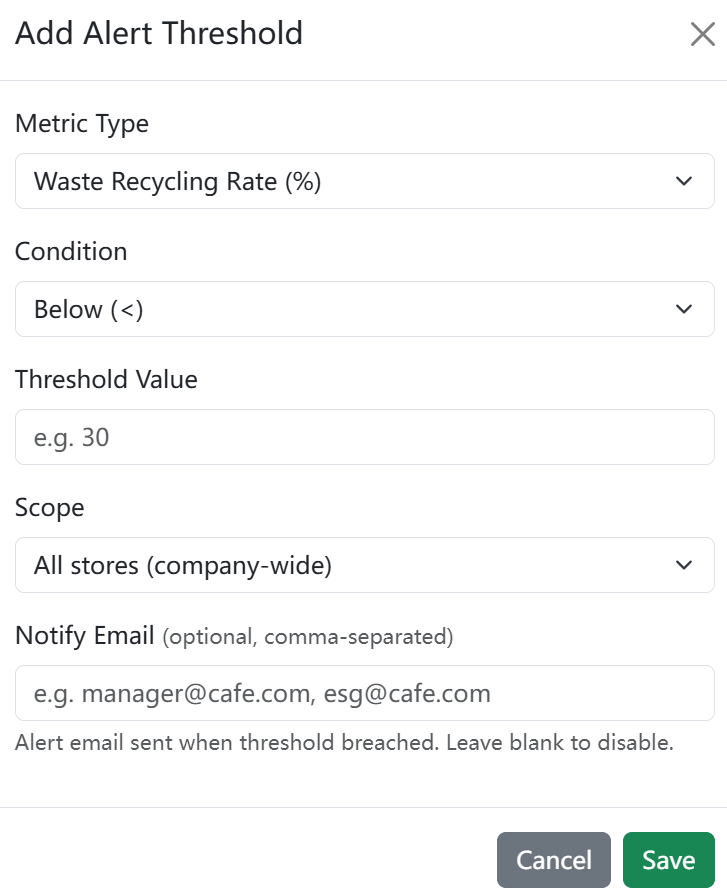
\includegraphics[height=5.5cm]{the Add Threshold modal.png}
  \caption{Alert Centre with active thresholds and logs (left) and threshold configuration form (right)}
  \label{fig:alerts-threshold}
\end{figure}


\subsection{ESG Governance (Supplier + Policy)}
Within ESG Management, HQ managers maintain two governance assets. \emph{Supplier ESG} lets managers create supplier records and complete the ESG scorecard by selecting 0/50/100 for each sub-indicator; the system then auto-computes dimension scores and the overall grade. \emph{Company Policy} is a lightweight internal document store: managers create, edit, and delete policies with title, category, status, effective date, version, and content, and open each in a detail view.

\begin{figure}[H]
  \centering
  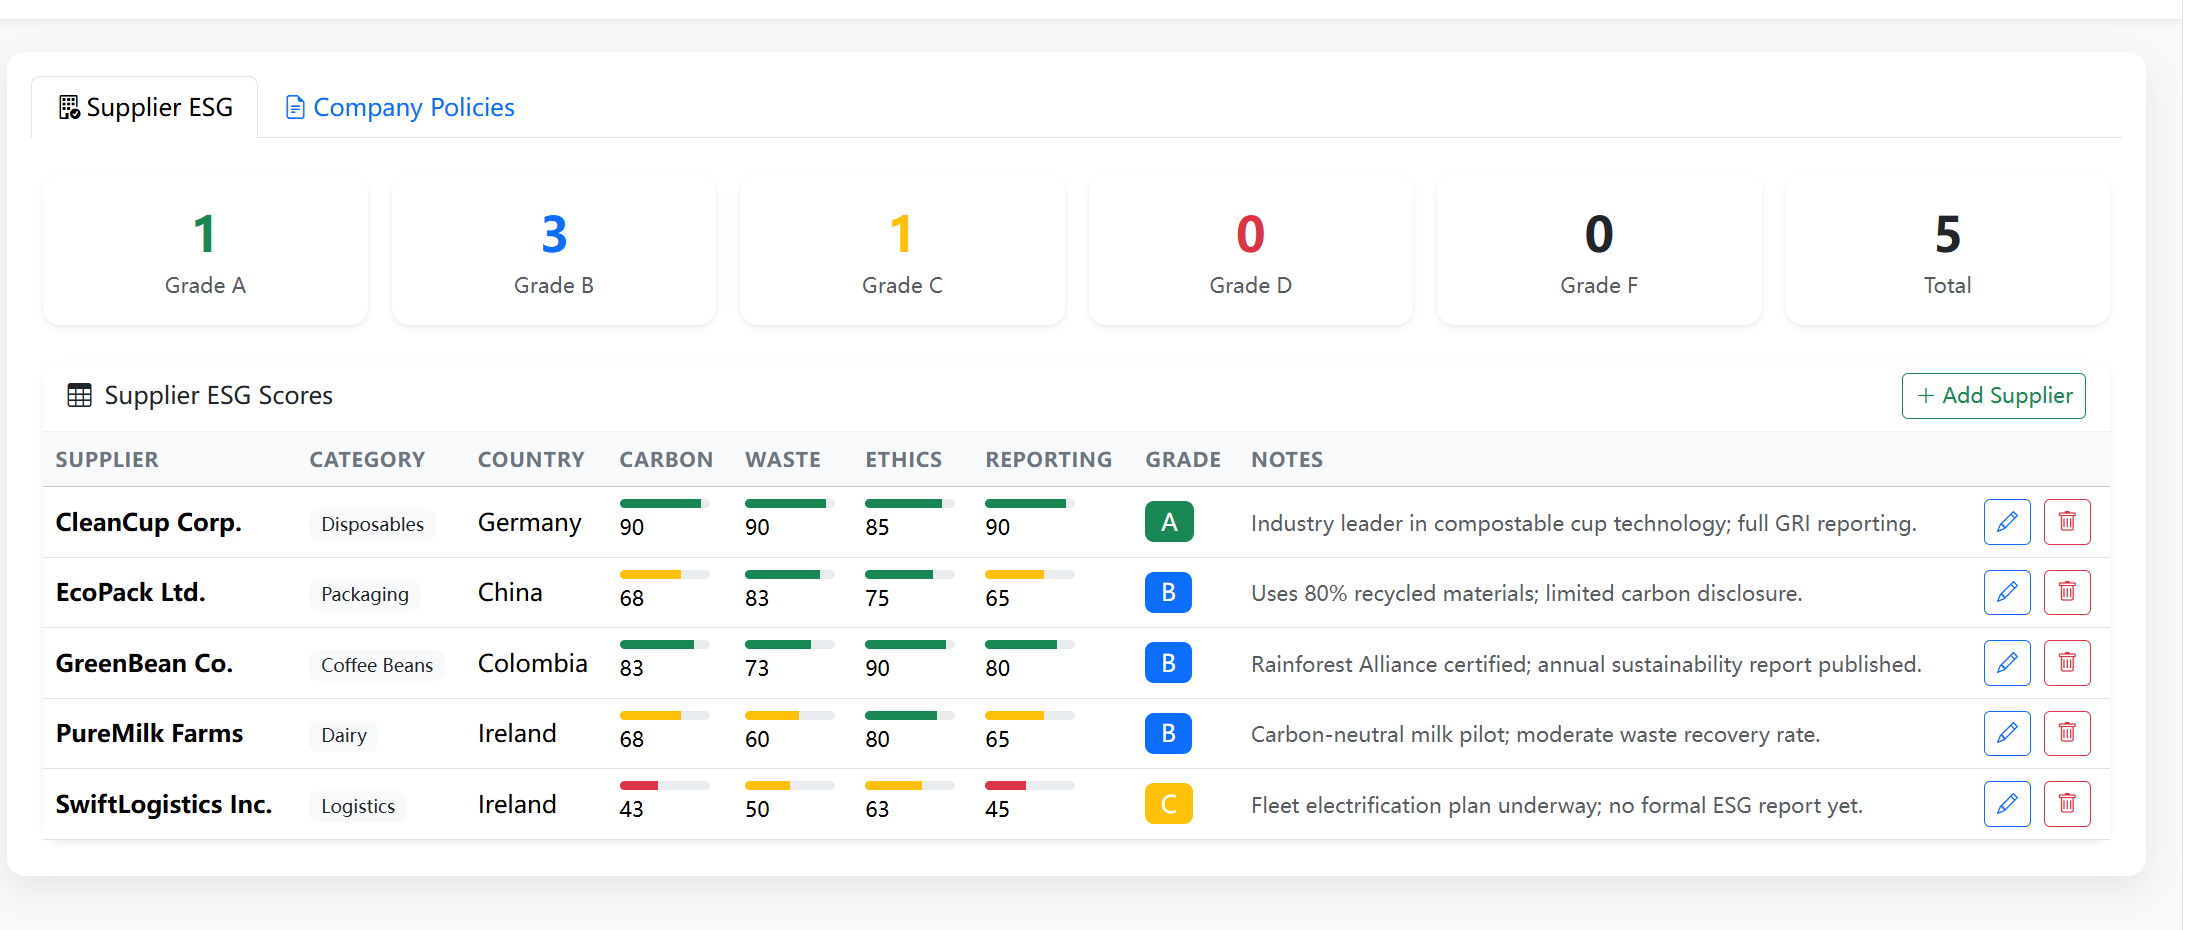
\includegraphics[width=0.82\textwidth]{supplier ESG table with grades visible.png}\\[0.4em]
  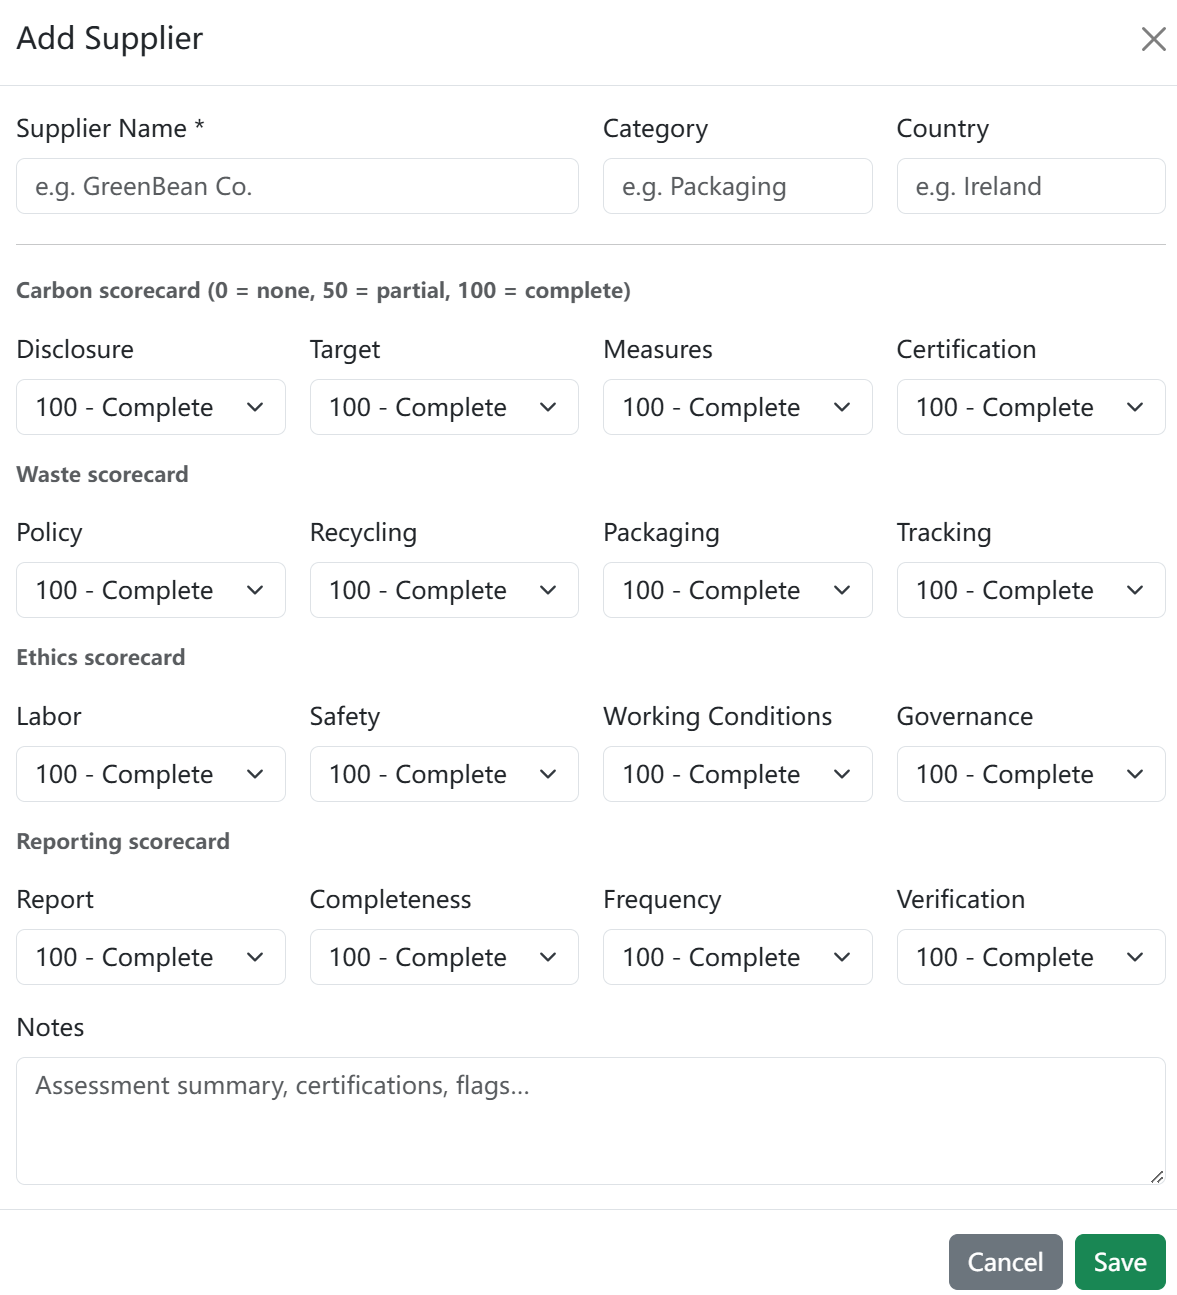
\includegraphics[width=0.42\textwidth]{add and edit supplier modal showing scorecard.png}
  \caption{Supplier ESG: scorecard table with grades and dimension scores (top), and the supplier scoring form (bottom)}
  \label{fig:esg-supplier}
\end{figure}

\begin{figure}[H]
  \centering
  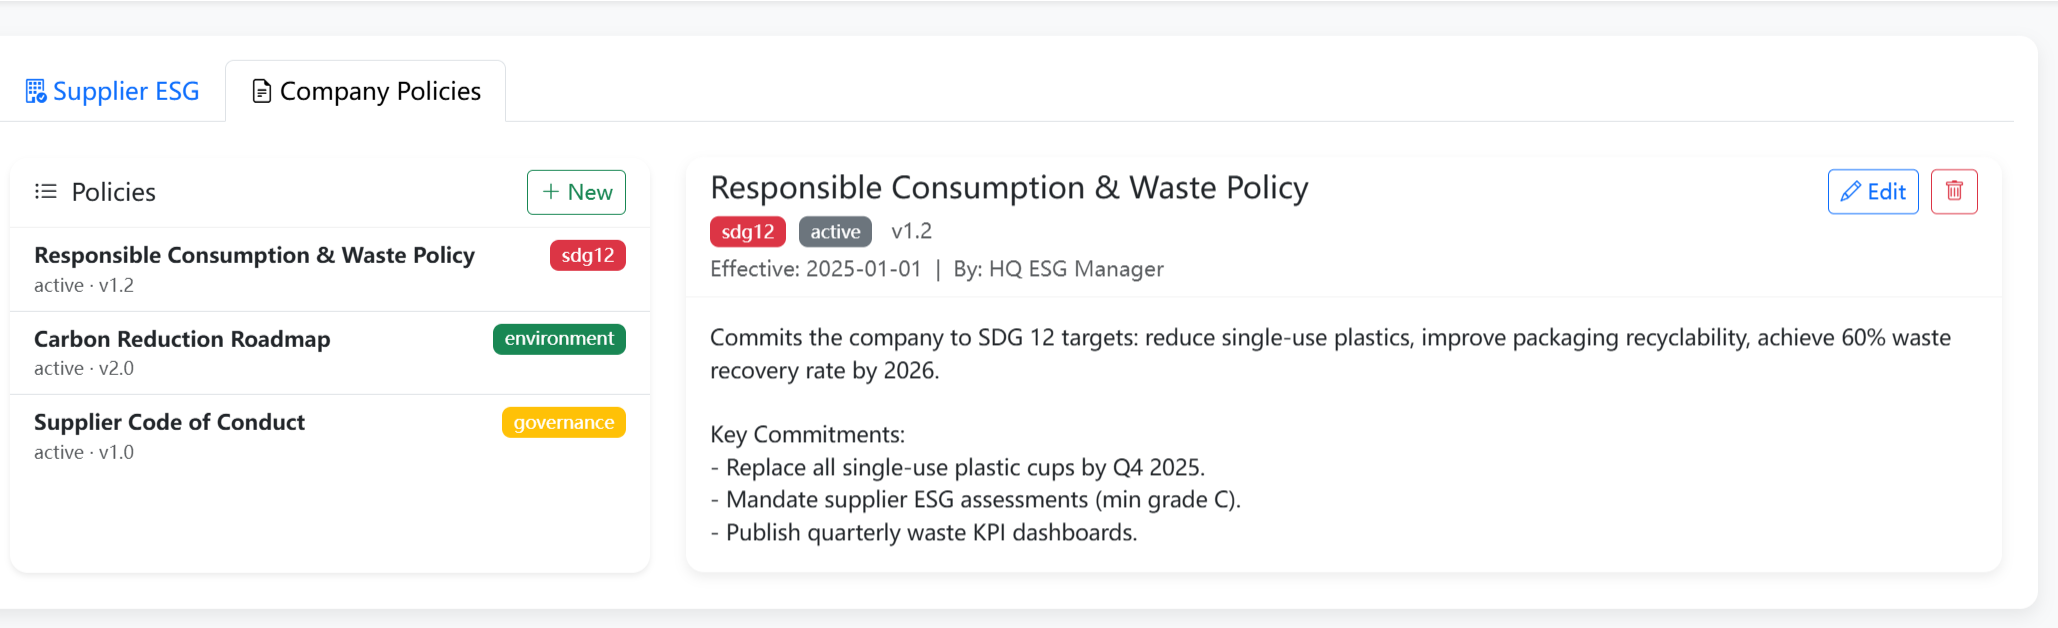
\includegraphics[width=0.65\textwidth]{the policy list.png}
  \caption{Company Policy management list with category, status, and effective-date metadata}
  \label{fig:esg-policy}
\end{figure}


\subsection{User Management}
The User Management page is accessible to HQ managers and admins. It provides summary cards for role distribution, a full user table with inline controls, and supports creating, editing, resetting passwords, and deleting accounts. Role and scope assignment -- including region and store fields -- can be configured when adding or editing a user.

\begin{figure}[H]
  \centering
  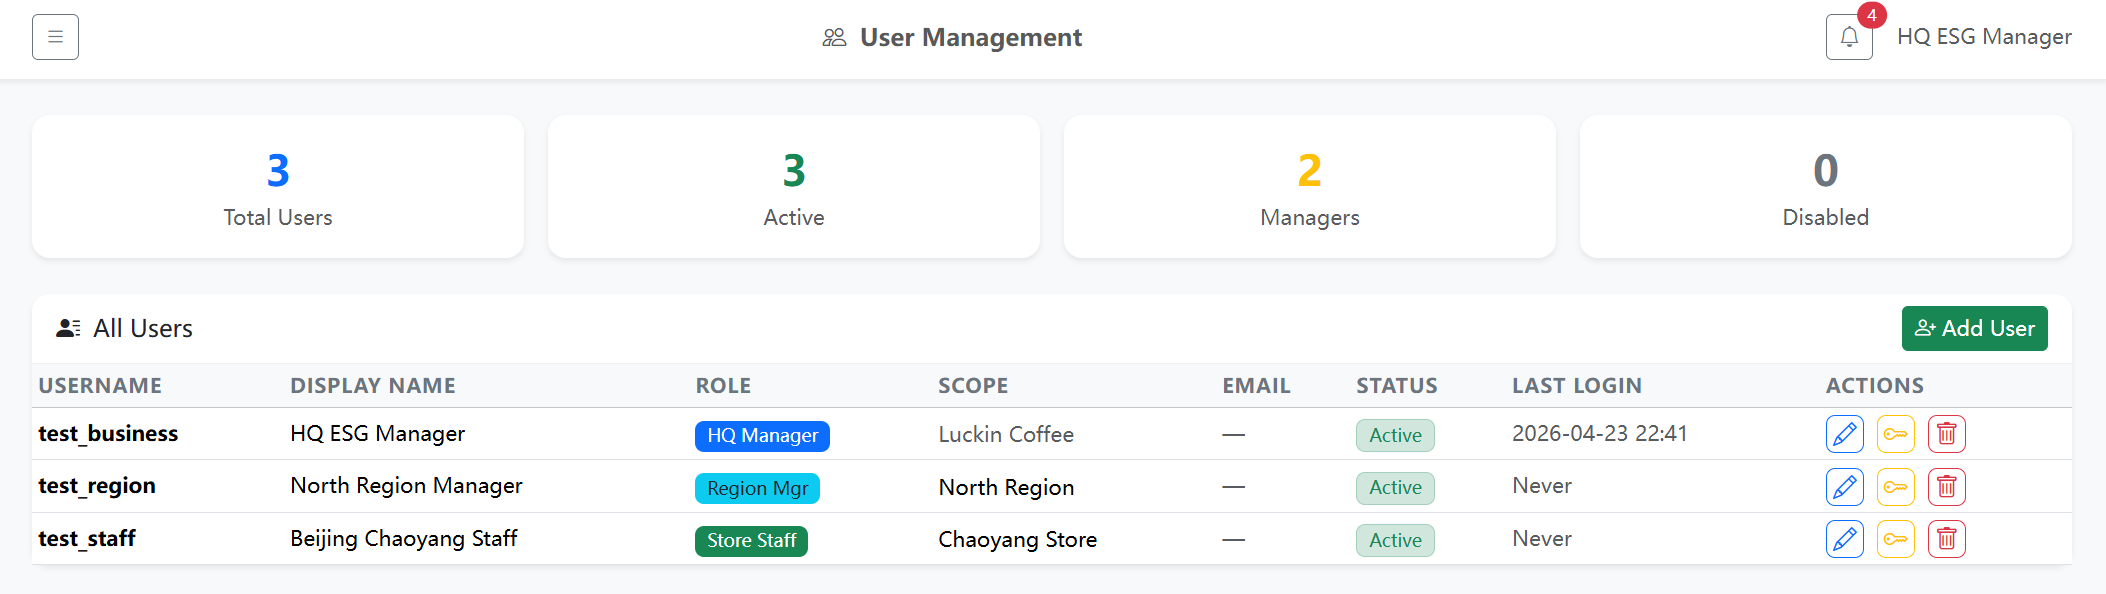
\includegraphics[width=0.88\textwidth]{main user table with summary cards.png}
  \caption{User management overview with role and scope summary cards}
  \label{fig:user-table}
\end{figure}


\subsection{Audit Log}
The Audit Log page enhances management visibility into critical system operations, with a focus on supporting review and accountability. It includes summary cards, filters, and an operation table that displays key details—including time, user, role, action, target, detail, and IP address—allowing managers to easily inspect and review system activity.
\begin{figure}[H]
  \centering
  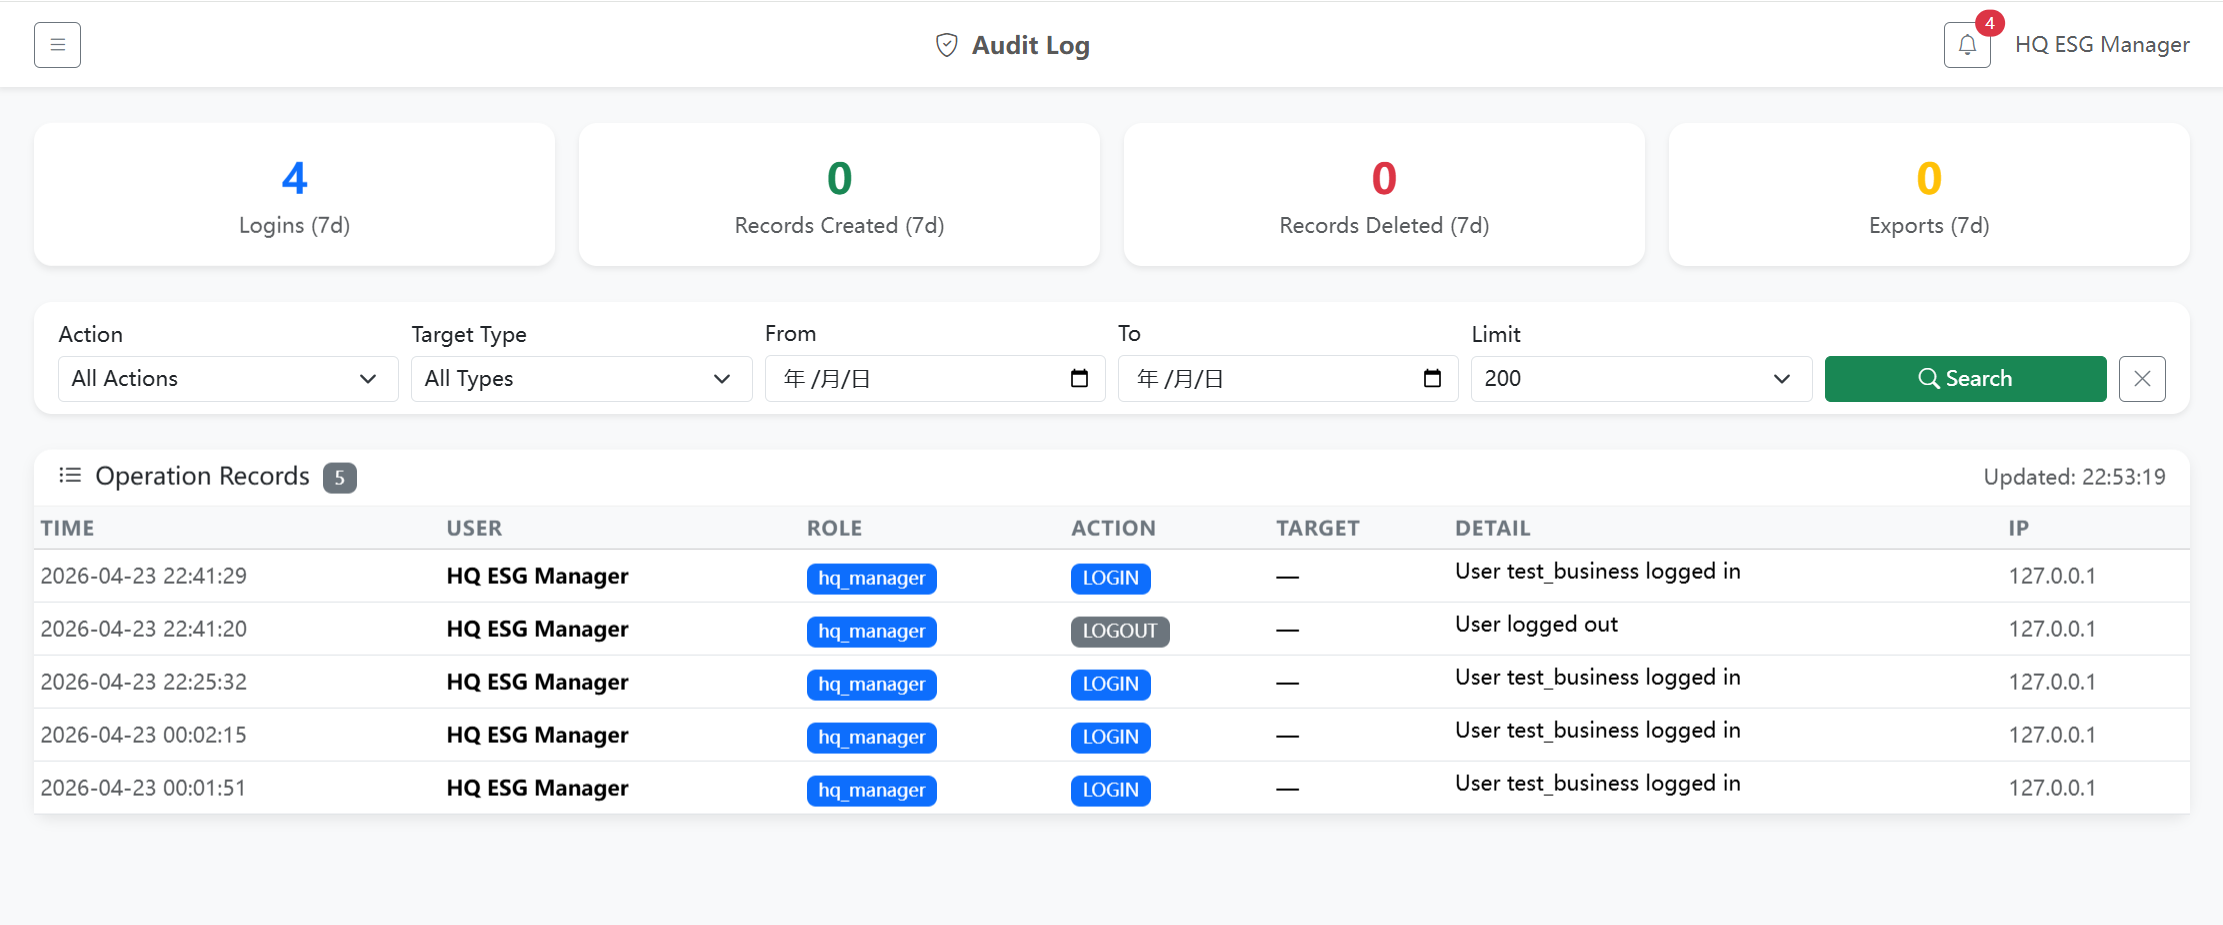
\includegraphics[width=0.65\textwidth]{the Audit Log page.png}
  \caption{Audit log with filters and activity table}
  \label{fig:audit-log-page}
\end{figure}

\section{Admin Guide}\label{sec:admin}

Administrators hold the broadest authority on the platform. They share most management pages with HQ managers (see Section~\ref{sec:hq}), but their data scope is platform-wide rather than company-bound. The three differentiators that matter most during testing are:

\begin{itemize}[leftmargin=1.4em,itemsep=2pt,topsep=2pt]
    \item \textbf{Platform-wide user management} -- create, edit, reset passwords, and delete accounts across any company, not just one. The user table and summary cards described in Section~\ref{sec:hq} therefore show every account in the system.
    \item \textbf{Cross-company audit visibility} -- the Audit Log page returns activity from every company, with the same filters and export options as the HQ-scoped view.
    \item \textbf{System Health card on the dashboard} -- an Admin-only widget showing active user counts, audit activity over the last twenty-four hours, and the open-alert backlog across the platform (see Figure~\ref{fig:role_dashboards}, bottom panel).
\end{itemize}

Because admins reuse the same management pages as HQ managers, this guide does not repeat their interaction details. The most common admin tasks during testing -- creating a cross-company user, searching the audit log, and inspecting system health -- are listed in Section~\ref{sec:tutorial}.


\section{Hands-On Tutorial for New Users}\label{sec:tutorial}
\new{This section provides a concise hands-on walkthrough for first-time evaluators. Open the platform URL in any modern browser and log in with one of the four pre-configured accounts (Section~2.2); the platform ships with a 218-store demonstration dataset, so every role-specific page contains realistic data immediately after first login. Table}~\ref{tab:walkthrough}\new{ lists one short scripted task per major function, grouped by role; each task should complete within 1--2 minutes on the demo dataset.}

\begin{table}[H]
\centering
\scriptsize
\begin{tabularx}{\linewidth}{@{}p{0.08\linewidth}p{0.20\linewidth}Xp{0.22\linewidth}@{}}
\toprule
\textbf{Role} & \textbf{Task} & \textbf{Steps (1--3)} & \textbf{Expected Outcome} \\
\midrule
Staff  & Log a carbon record    & Carbon $\to$ Add $\to$ fill category/quantity $\to$ Submit              & New row at top of table; dashboard KPI updates       \\
Staff  & Log a waste record     & Waste $\to$ Add $\to$ category/total/recycled $\to$ Submit             & Row inserted; recycle-rate KPI refreshes             \\
Region & Review regional alerts & Alerts $\to$ filter by region $\to$ click a row                        & Alert detail visible; cross-link to source record    \\
Region & Region leaderboard     & Dashboard $\to$ Region Leaderboard card                                & Stores ranked by recycling rate and carbon intensity \\
Region & Monthly comparison     & Carbon $\to$ Compare $\to$ pick month                                  & Bar of this/last month and regional average          \\
Region & Inspect store map      & Map $\to$ filter region $\to$ click a red marker                       & Popup with YTD carbon, recovery rate, alert count    \\
HQ     & Add threshold rule     & Alerts $\to$ Add Threshold $\to$ metric/condition/value                & Threshold appears in active list                     \\
HQ     & Score a supplier       & ESG Mgmt $\to$ Supplier $\to$ pick supplier $\to$ score                & Sub-indicator scores recomputed; grade letter updates\\
HQ     & Generate AI report     & Reports $\to$ keep AI toggle on $\to$ Generate                         & Report row with AI badge; PDF export available       \\
Admin  & Create a user          & User Management $\to$ Add $\to$ role/scope $\to$ Save                  & New row in users table; account can log in           \\
Admin  & Audit log search       & Audit Log $\to$ filter user/action $\to$ Apply                         & Matching events visible with time/IP/target          \\
Admin  & Inspect system health  & Dashboard $\to$ System Health card                                     & Active users / open alerts / recent activity shown   \\
\bottomrule
\end{tabularx}
\caption{Hands-on task walkthroughs across four roles (12 representative tasks)}
\label{tab:walkthrough}
\end{table}

\new{The seeded demo dataset includes 218 stores distributed across regions. To quickly find pages with non-trivial data, testers can target one of four engineered groups: \textbf{spike stores} (single large carbon entries), \textbf{silent stores} (no submissions in the latest period, triggering data-gap alerts), \textbf{high-alert stores} (multiple recent threshold breaches), and \textbf{outlier stores} (waste-recycling ratios outside the regional norm). Store IDs for each group are listed in the project's seed-data documentation; targeting them yields more meaningful exploration than browsing arbitrary stores.}


\section*{Conclusion}
This manual has covered the platform from login through to role-specific workflows, organised across four user types: Store Staff, Region Manager, HQ Manager, and Admin. Each role accesses a tailored set of pages, and the shared workflow sections in Section~4 provide the operational foundation that applies across all roles. Users conducting system testing should refer to the test accounts in Section 2.2 and follow the relevant role chapter as a step-by-step guide. \new{New users may also follow Section}~\ref{sec:tutorial}\new{ as a guided walkthrough.}
\bibliographystyle{unsrtnat}
\bibliography{refs}

\end{document}
